\documentclass[a4paper,12pt]{elsarticle}
% vim: tw=0 wm=0

\setcounter{tocdepth}{3}
\usepackage{amssymb}
\usepackage{amsmath}
\usepackage{multirow}
\usepackage{longtable}
\usepackage{comment}
\usepackage{placeins}
\usepackage{mathtools}
\usepackage{algorithm}
\usepackage{algpseudocode}
\usepackage{enumitem}
\usepackage[utf8]{inputenc}
\usepackage{booktabs}
\usepackage{array}
\usepackage[pdfencoding=auto,psdextra]{hyperref}
\usepackage{booktabs}
\usepackage{bookmark}% faster updated bookmarks
\usepackage{hypcap} % fix the links
\evensidemargin\oddsidemargin
\usepackage{graphicx}
\pagestyle{plain}
\usepackage{xcolor}
\newcommand\ToDo[1]{\textcolor{red}{#1}}
\usepackage{tabularx}
\usepackage{xspace}
\usepackage{color}
\usepackage{epsfig}
\usepackage{caption}
\usepackage{subcaption}
\usepackage{mathrsfs}
\usepackage{amssymb}
\usepackage{amsmath}
\usepackage{amsthm}
%\usepackage{changes}
\usepackage{tikz}
\usepackage{fullpage}
\usepackage{calc}
\usetikzlibrary{positioning,shadows,arrows,trees,shapes,fit}
\usepackage{blindtext}
\usepackage{pgfplots}
\pgfplotsset{compat=1.16}

\usepackage{numprint}
\npdecimalsign{.}
\npthousandsep{}

\usepackage[draft,nomargin,inline]{fixme}
\fxsetface{inline}{\itshape}
\fxsetface{env}{\itshape}
%\fxuselayouts{margin}
%\fxuselayouts{inline}
\fxusetheme{color}

\usepackage{url}
\newcommand{\keywords}[1]{\par\aDSvspace\baselineskip
	\noindent\keywordname\enspace\ignorespaces#1}

\usepackage{tikz}
\usetikzlibrary{positioning}
\definecolor{canaryyellow}{rgb}{1.0, 0.94, 0.0}
\definecolor{brightgreen}{rgb}{0.4, 1.0, 0.0}
\definecolor{jazzberryjam}{rgb}{0.65, 0.04, 0.37}

%defining of command

\newcommand\floor[1]{\lfloor#1\rfloor}
\newcommand\ceil[1]{\lceil#1\rceil}
\newcommand\str[1]{\texttt{#1}}
\newcommand\pL[1][]{\ensuremath{p^{\mathrm{L}#1}}}
\newcommand\pR[1][]{\ensuremath{p^{\mathrm{R}#1}}}
\newcommand\qL{\ensuremath{q^\mathrm{L}}}
\newcommand\qR{\ensuremath{q^\mathrm{R}}}
\newcommand\pLH{\ensuremath{\hat{p}^\mathrm{L}}}
\newcommand\pRH{\ensuremath{\hat{p}^\mathrm{R}}}
\newcommand{\Vext}{\ensuremath{V_\mathrm{{ext}}}}
\newcommand\UB{\ensuremath{\mathrm{UB}}}
\newcommand\Sigmand{\ensuremath{\Sigma^\mathrm{nd}}}
\newcommand{\mdmwnpp}{MDMWNPP\xspace}

\renewcommand{\labelenumii}{\theenumii}
\renewcommand{\theenumii}{\theenumi.\arabic{enumii}.}
\setlength{\leftmarginii}{1.8ex}
\raggedbottom
\algnewcommand\algorithmicforeach{\textbf{for each}}
\algdef{S}[FOR]{ForEach}[1]{\algorithmicforeach\ #1\ \algorithmicdo}

% scaling factor for tables
\newcommand\tabscale{0.8}
\newtheorem{definition}{Definition}
\newtheorem{Lemma}{Lemma}

\begin{document}
	
	%\setlength{\parindent}{0pt}  % disallow indentations
	%\numberwithin{table}{1}
	%\mainmatter  % start of an individual contribution
	
	% first the title is needed
	\title{\textsc{Rils}-\textsc{Rols} : Robust Symbolic Regression via Iterated Local Search and Ordinary Least Squares}
	
	\author[1]{Aleksandar Kartelj}
	\author[2]{Marko Djukanovi\'c}
	\address[1]{$kartelj@matf.bg.ac.rs$, \\  Faculty of Mathematics, University of Belgrade, Serbia}
	\address[2]{$ marko.djukanovic@pmf.unibl.org$,\\   Faculty of Natural Sciences and Mathematics, University of Banja Luka, Bosnia and Herzegovina}
	\begin{abstract}
		In this paper, we solve the well-known, prominent  Symbolic regression problem, intensively studied within the last two decades. This problem has a wide range of applications;  for example, the obtained SR models could serve theoretically, providing insight towards establishing physical theory behind, thus helping to establish reasonable hypotheses.  Practical applications include revealing complex ecological dynamics in ecology, discovering mutations effects on protein stability in biology, modelling analytic representations of the exciton binding energy in energy science,   finding models for band gaps of NaCl-type compounds
		in material science, just to name a few. We propose a new meta-heuristic-based approach, called \textsc{Rils}-\textsc{Rols} algorithm to solve the problem of Symbolic regression. There are several key concepts utilized within this algorithm: ($i$) Iterated local search scheme is used as the backbone; ($ii$) ordinary least square method is used in the search to make it efficient with  determining the best--fitting   coefficients in considered solutions (models);  ($iii$) a novel fitness function is utilized which combines the three known measures: $R^2$ score, RMSE score, and the size of the model which is weighted by a parameter. The experiments are conducted on the two ground-truth benchmark sets, \textsc{Feynman} and \textsc{Strogatz} comparing \textsc{Rils}-\textsc{Rols} algorithm to 14 other competitors from the literature where different levels of the Gaussian white noise in the input data are utilized.  Our method obtains new best exact percentages on both benchmark sets compared to other literature approaches regardless of varying the level of nose. Moreover, a new unbiased randomly generated set of problem instances are introduced where the scalability of our method is thoroughly demonstrated in terms of various instance properties. 
	\end{abstract}
	\maketitle
	
	
	\section{Introduction}\label{sec:introduction}
	
	The problem of symbolic regression (SR)~\cite{billard2002symbolic} has attracted many researchers over the last decade to study it intensively. SR can be seen as a generalization of the well-known concept of linear regression, i.e., polynomial regression~\cite{stimson1978interpreting}. All regression models in principle have the same task: given a set of $n$-dimensional input data and the output data, the aim is to find a  mathematical expression (function) consisting of $n$ (input) variables that fit the output data w.r.t. some in advance known measure.  This computationally intensive task is in general provenly NP--hard~\cite{virgolin2022symbolic}. When aiming a model to be a linear combination of input variables, it represents the problem of linear regression. However, when there are some nonlinear relations between variables, which are relevant, linear regression models are not enough. This is the point where symbolic regression comes into play. Unlike linear regression, it allows the search over the space of all possible mathematical formulas to find the best-fitting ones able to predict the output variable from the input variables. The basis of constructing the explicit formula is the basic operations like addition and multiplication, as well as polynomial, trigonometric, exponential, and other elementary functions.  
	%Application: https://towardsdatascience.com/real-world-applications-of-symbolic-regression-2025d17b88ef
	
	Concrete examples of the application of SR include obtaining a less black--box tool, as it may say more about how SR models achieve predictions, that is the coefficients and functions that build the model may indicate on larger importance of some variables over the others. Moreover, in that way, we may grasp why the variables are related in the obtained way. As an example, the appearance of an exponential function may associate with some physical phenomenon such as the intensity of radiation or acceleration over time, see~\cite{udrescu2020ai}. Additionally, the SR models, if they are correct, may possess larger extrapolation power than other mathematical models, especially better from the neural network--based methods. SR models may maximize obtaining physically more reasonable equations that could serve as an insight towards establishing physical theory behind as the final goal.  Practical applications of SR in chemical and biological sciences are listed in~\cite{weng2020simple}. In particular,  the discovery of a series of new oxide perovskite catalysts with improved activities can be found there. The application of SR to discovering physical laws from a distorted video is studied in~\cite{udrescu2021symbolic} by means of an unsupervised learning method. Revealing complex ecological dynamics by SR is presented in~\cite{chen2019revealing}, tackled by a machine learning method. Application of SR to model the effects of the mutations on protein stability, in the domain of fundamental and applied biology,  is shown in~\cite{louis2021reviewing}. One of the recent work studies of auto-discovering conserved quantities using trajectory data from unknown dynamical systems, where SR is solved by a machine learning algorithm, see~\cite{liu2021machine}. Last but not least, we mention the paper~\cite{liang2019phillips} which discovers the application of SR to model analytic representations of the exciton binding energy. The use of solving the SR in material science is described in~\cite{wang2019symbolic,wang2022symbolic,burlacu2022symbolic,kabliman2021application}. Yet another application to wind speed forecasting is given in~\cite{abdellaoui2021symbolic}. 
	
	There are many different ways to tackle the SR by achieving the right analytic expressions, most of them are related to machine learning techniques or the technique of genetic programming (GP) and various approximate methods, such as meta-heuristics. Among the first GP methods to tackle SR is the one of Raidl~\cite{raidl1998hybrid} based on a hybrid variant of genetic programming. A differential evolution algorithm was proposed by Cerny et al.~\cite{cerny2008using}. Age-fitness Pareto Optimization approach is proposed by Smidt and Lipson~\cite{schmidt2010age}.  Application of the artificial bee colony programming to solve SR is proposed by Karaboga et al.~\cite{karaboga2012artificial}. 
	The influence of local--based heuristics on solving SR is reported by Commenda in his PhD thesis~\cite{kommenda2018local}. A  GP-based approach, the gene-pool optimal mixing evolutionary algorithm (\textsc{Gomea}) is studied by Virgolin et al.~\cite{virgolin2021improving}.  Another evolutionary algorithm, the interaction-transformation EA (\textsc{Itea}) has been proposed by de Franca et al.~\cite{de2021interaction}. Simulated annealing to solve SR is proposed by Kantor~\cite{kantor2021simulated}. A Variable neighbourhood programming approach to solve SR  is proposed by Elleurich et al.~\cite{elleuch2020variable}; this technique is initially proposed in~\cite{elleuch2016variable}. 
	Kommenda et al.~\cite{kommenda2020parameter} proposed a method called \textsc{Operon} algorithm, which uses nonlinear least squares for parameter identification of SR models further integrated into a local search mechanism in tree-based GP. The C++ implementation of \textsc{Operon} is discussed in~\cite{burlacu2020operon}. The method that utilizes the Taylor polynomials to approximate the symbolic equation that fits the dataset, called Taylor genetic programming, is proposed in~\cite{he2022taylor}. A GP approach that uses the idea of semantic back-propagation (Sbp-Gp) is proposed in~\cite{virgolin2019linear}.   Empirical analysis of variance between many GP--based methods for SR is discussed in~\cite{kammerer2021empirical}. It is also worth mentioning the GP--based Eurequa commercial solver~\cite{schmidt2009distilling, schmidt2011machine} that uses age-fitness pareto optimization with co-evolved fitness estimation. This solver is nowadays accepted as the gold standard of symbolic regression. 	  
	
	
	Machine learning--based method based on Bayesian symbolic regression (\textsc{Bsr}) is proposed in~\cite{jin2019bayesian},  belongs to the family of Markov Chain Monte Carlo algorithms. Deep Symbolic Regression (\textsc{Dsr}), an RNN approach, is proposed in~\cite{petersen2019deep} utilizing the policy gradient search. This mechanism of search is further investigated in~\cite{landajuela2021improving}. A fast neural network approach, called \textsc{OccamNet},  is proposed in~\cite{costa2020fast}.  A deep reinforcement learning approach enhanced with genetic programming is given in~\cite{mundhenk2021symbolic}. 
	
    Powerful hybrid techniques to solve SR are also well studied; among them, we emphasize the \textsc{Eplex} solver from~\cite{la2019probabilistic,la2016epsilon} and AI Feynman algorithm from~\cite{udrescu2020ai}, a physics-inspired divide-and-conquer method combined with the neural network fitting. The latter is one of the most efficient methods for physically inspired models. We also mention the Fast Function Extraction (\textsc{Ffx}) algorithm developed by McConaghy~\cite{mcconaghy2011ffx},  which is a non-evolutionary method   combined with a machine learning technique---path-wise regularized learning--- which prunes quickly a huge set of candidate basis functions down to compact models.
	
	A short overview of the most important literature methods to solve SR is given in Table~\ref{tab:gp-based} in the chronological order of their appearances.  
	
	
	\begin{table}[!ht]
		\centering
		\scalebox{0.7}{
			\begin{tabularx}{550pt}{l  l  X}  
				Algorithm          &   Paper/year &   Short details   \\ \hline
				\textsc{Gp}        &    \cite{koza1994genetic} (1994)    & Application of GP to SR \\ 
				\textsc{Hybrid-Gp}  &   \cite{raidl1998hybrid} (1998)   & GP--based method; solutions locally optimizes by method of least squares to find optimum coefficients for top-level terms \\ 
				\textsc{Dfe}        & \cite{cerny2008using} (2008)   & Differential evolution algorithm \\
				\textsc{Apf-Fe}                & \cite{schmidt2009distilling, schmidt2011machine} (2009, 2011) & Age-fitness pareto optimization approach using co-evolved fitness estimation   \\
				APF            &      \cite{schmidt2010age} (2010)        &  Age-fitness pareto optimization approach                        \\
				\textsc{Ffx}  & \cite{mcconaghy2011ffx} (2011)  & The Fast Function Extraction algorithm --  non-evolutionary technique based on a machine learning technique called path-wise regularized learning \\
				\textsc{Abcp} &  \cite{karaboga2012artificial} (2012)  & Artificial bee colony programming  approach \\
				\textsc{Eplex}          &      \cite{la2016epsilon} (2016)         &   A parent selection method called $\epsilon$--lexicase selection  \\ 
				\textsc{Mrgp} & \cite{arnaldo2014multiple} (2014) & It decouples and
				linearly combines a program's subexpressions via multiple regression on the target variable  \\
				Local optimization NLS    & \cite{kommenda2018local} (2018)   & Constants Optimization in GP by Nonlinear Least Square \\
				\textsc{Feat} & \cite{la2018learning} (2018) & Features are represented as networks of multi-type expression trees  comprised of activation functions; Differentiable features are trained via gradient descent \\
				\textsc{Sbp-Gp} &  \cite{virgolin2019linear} (2019)  & The idea of semantic back-propagation utilized in GP \\
				\textsc{Bsr} & \cite{jin2019bayesian} (2019) & ML--based approach; Bayesian symbolic regression  \\ 
				\textsc{Dsr}  & \cite{petersen2019deep} (2019) & Deep Symbolic Regression based on a RNN approach further utilizing the policy gradient search \\
				\textsc{Operon} & \cite{kommenda2020parameter} (2020) &  Utilizing nonlinear least squares for parameter identification of SR models with LS \\
				\textsc{Vnp}    & \cite{elleuch2020variable} (2020) & VNS based GP approach \\
				\textsc{OccamNet} & \cite{costa2020fast} (2020) &   A fast neural network approach; the model defines a probability distribution over a non-differentiable function space; it samples functions and updates the weights with back-propagation  based on cross-entropy matching in an EA strategy	 \\
				
				\textsc{AI-Feynman} & \cite{udrescu2020ai} (2020) & A physics-inspired divide-and-conquer method; it  combines neural network fitting \\
				\textsc{Gomea}  & \cite{virgolin2021improving} (2021)    & A model-based
				EA framework called Gene-pool optimal mixing evolutionary algorithm \\
				\textsc{Itea} & \cite{de2021interaction} (2021)   & EA based approach called the interaction-transformation EA   \\
				\textsc{Sa} & \cite{kantor2021simulated} (2021) &  Simulated annealing approach \\
				
				\textsc{Drla} & \cite{mundhenk2021symbolic} (2021)  &    A deep reinforcement learning approach enhanced with genetic programming \\
				\textsc{Taylor-Gp} &  \cite{he2022taylor} (2022)  &  Taylor polynomials approximations  \\ \hline
				
				
		\end{tabularx} }
		\caption{Overview of methods to solve SR.}
		\label{tab:gp-based}
	\end{table}
	
	
   The progress in the SR field suffered from a lack of uniform, robust, and transparent
	benchmarking standards over the last two decades. Recently, La Cava et al.~\cite{la2021contemporary} proposed an
	open-source, reproducible benchmarking platform for SR, called SRBench. The authors extended  PMLB~\cite{olson2017pmlb},  a repository of standardized regression problems, by 130 SR datasets for which model forms are known; see more in the aforementioned paper. In the extensive experimental evaluation  where 14
	symbolic regression methods and 7 machine learning methods are compared on the set of 252 diverse regression problems. The general conclusions derived from there are: ($i$) when comes to real-world problems, the best performing algorithms are those which combine genetic algorithm with a parameter estimation; ($ii$) when comes to the instances with a presence of noise, the GP--based and deep learning techniques are performing similarly.  
	
	In this work we present a novel approach to solve SR, which combines the popular iterated local search meta-heuristic (ILS)~\cite{lourencco2003iterated,lourencco2019iterated} with the ordinary least square  method (OLS)~\cite{leng2007ordinary}. Briefly, ILS handles combinatorial (discrete) aspects of search space, while OLS helps in the process of a coefficient determination, so it handles continuous parts of the search space. As will be shown later, the proposed method has shown its robustness w.r.t. introduced noise, therefore we called the method \textsc{Rils}-\textsc{Rols}  (with letters R corresponding to regression and robust).    Additionally, in order to navigate the search towards not only accurate models, but increasing the chances to get the exact one, the algorithms is equipped with a carefully constructed fitness function that utilizes three important scores of a solution (model): RMSE and $R^2$ scores which participate into models accuracy, and a weighted solution size that will contribute penalizing large (mostly non-exact) solutions. 
	
	The main contributions of this work may be summarized as follows: 
	
	\begin{enumerate}
		\item The proposed method outperforms all (14) state-of-the-art methods for ground-truth problems from literature, considered in the SRBench benchmark.  
		
		\item The method shows its high robustness, which is proved by comparison to other algorithms under different levels of Gaussian white noise. 
		
		\item The method is very efficient, taking in average around xyz seconds to reach exact solution -- when exact solution is found. \fxnote{Ovo treba dodati u eksp. sekciji...}
		
		\item New set of unbiased instances is   introduced that are randomly generated formula of various sizes and number of input variables in exact models. This set was employed to methodologically analyze the influence of formula size, number of input variables and noise on the solving difficulty. 
	\end{enumerate}
	
	
	\section{Problem definition and search space}
	\label{sec:search-space}
	In this section we formally define the SR problem, followed by defining the search space framework of the problem.  
	
	\begin{definition}
		Given is a dataset $D = \{(x_i, y_i)\}_{i=1}^n$, where $\textbf{x} \in \mathbb{R}^d$ represents input variables (features), and $y$ target variable. Suppose that there exists an analytical model of the form $f(\textbf{x})= g^*(\textbf{x}, \theta^*) + \epsilon $ that is a generator of all observations from $D$.  
		The goal of SR is to learn a mapping $\tilde{f}(\textbf{x})=  \tilde{g}(\textbf{x}, \tilde{\theta})  \colon \mathbb{R}^d \mapsto \mathbb{R}$  estimated by searching through the space of (mathematical) expressions  $\tilde{g}$ and parameters $\tilde{\theta}$ where  $\epsilon$ is the presented  white noise within the given input data. 
		
	\end{definition}
	
	Koza~\cite{koza1994genetic} introduced the problem of SR as a specific application of genetic programming. GP deals with the object called programs, which need to be optimized. In particular, the programs are represented by syntax trees consisting of functions/operations over input features and constants; as an example of a function represented by a syntax tree, see Figure~\ref{fig:syntax-tree-example} In essence, syntax trees are elements of the search space of SR. That is, each sample model $\tilde{f}$ may be seen as a point in the search space, represented by respective syntax tree. How accurate is this mapping, we compute on the basis of the historical data $D$ and the chosen error   measure (such as $MSE$, or $R^2$). Interestingly, the search space of SR consists of its discrete and continuous part. More precisely, the model we are seeking for might be obtained as a composition of some functions from a (finite) set of mathematical functions. It is common to use the set of the following elementary mathematical functions in the experiments: $\sqrt{x}, x^2 $, $\sin$, $\cos$, $\log$, $\exp$, $\arcsin$, $\arccos$, and $a^x$. It is allowed to link functions will all four operators: $+$, $-$, $\times$, and $/$. After fixing functions that build models, the set of optimal coefficients that  fits to this model must be provided. For the most physical models, these coefficients may receive any real value, that is they are continuous in its nature. 
	
	\begin{figure}[!ht]
		\centering
		\begin{tikzpicture}
			[font=\small, edge from parent, 
			every node/.style={top color=white, bottom color=blue!25, 
				rectangle,rounded corners, minimum size=6mm, draw=blue!75,
				very thick, drop shadow, align=center},
			edge from parent/.style={draw=blue!50,thick},
			level 1/.style={sibling distance=3cm},
			level 2/.style={sibling distance=1.2cm}, 
			level 3/.style={sibling distance=1cm}, 
			level distance=2cm,
			]
			\node (A) {$\times$} 
			child { node (B) {$\sin$}
				%child { node {x} 
					%edge from parent node[left=.5em,draw=none] {} }
				child { node {$x$}}
			}
			child {node (C) {$\times$}
				%child { node {x}
					%	child { node {C1a}}
					%}
				child { node {$x$}}
				child { node {$/$}
					child { node {$x$}}
					child { node {$y$} %edge from parent node[right=.5em,draw=none] {$\frac{a}{b}$}
					}
				}
			};
			%	child { node {+} 
				%	child { node {2}}
				%	child { node {$x$}}
				%};
			
		\end{tikzpicture}
		
		\caption{Syntax tree representation for the expression $\sin x \times   ( x \times  x / y  )  = \frac{x^2 \sin x }{y}$}
		\label{fig:syntax-tree-example}
	\end{figure}
	
	%\section{Literature review}\label{sec:lit-rev}
	
	
	\section{The proposed method}\label{sec:rils}
 
	Before we give details on our \textsc{Rils}-\textsc{Rols}  method for solving SR, we will explain the basics of two main techniques incorporated into our algorithm. These are ILS meta-heuristic and OLS methods. 
	
	\subsection{Iterated local search}
	Iterated local search (ILS)~\cite{lourencco2003iterated} is an efficient meta-heuristics, whose essential idea is given as follow. Iteratively generate a sequence of solutions produced by the (embedded) heuristic, such as local search or randomized greedy heuristics. When the search gets \emph{stuck} in local optimum, a \emph{perturbation} is performed -- this step is usually non-deterministic. This simple idea appeared in the literature by Baxter~\cite{baxter1981local} in early 1980s, and, since then, has been  re-invented by many researches under different names; some of the following names were used: iterated descent search~\cite{baum1998iterated}, large-step
	Markov chains~\cite{martin1991large}, chained local optimization~\cite{martin1996combining}, or, in some cases, combinations of these~\cite{applegate2003chained}. 
	
	The most popular version of ILS is shown in Algorithm~\ref{alg:ils}. Note that we use this version of ILS as the backbone of our \textsc{Rils}-\textsc{Rols}  algorithm.
	
	\begin{algorithm}
		\begin{algorithmic}[1] 
			\State \textbf{Input}: problem instance
			\State \textbf{Output}: an approximate (feasible) solution 
			\State $s \gets$ \texttt{Initialize}$()$
			\State  $s \gets$ \texttt{LocalSearch}($s$)
			\While{\emph{stopping criteria is not met}}
			\State  $s' \gets$ \texttt{Perturbation}($s$)
			\State  $s' \gets$ \texttt{LocalSearch}($s'$)
			\State  $ s \gets$ \texttt{AcceptanceCriterion}($s, s'$)
			\EndWhile
			\State \Return $s$
		\end{algorithmic}
		\caption{An ILS framework from   literature.}
		\label{alg:ils}
	\end{algorithm}  
	
	An initial solution may be generated randomly or by using a greedy heuristic, which is afterwards, improved by local search. At each iteration, ILS applies three steps. First, the current incumbent solution is perturbed -- it is partially randomized. Next, the perturbed solution is improved by a LS procedure. Thirdly, the LS outcome is thereafter compared to the incumbent solution and the search us possibly moved to the new solution, with accordance to the chosen acceptance criterion. Sometimes, ILS incorporates a mechanism of tabu list, which prevents the search getting back to already visited solutions.  		 
	
	\subsection{Ordinary least square method}\label{sec:ols}
	Ordinary least square method (OLS) is a linear regression technique. It is based on applying the least-square method to minimize the square residual (error) sum  between actual and predicted values (given by the model). More precisely, given data $({X}=(X_1, \ldots, X_d)^T, y)$, the task is to determine linear mapping $\tilde{y} = k \textbf{x} + b$, that is coefficients (line slope) $k = (k_1, \ldots, k_d)$ and $b$ (intercept), so that $ \sum_{i} |\tilde{y}_i - y_i|^2 $ is minimized. This sum is also know as the sum of squared error (SSE). There are many methods to minimize SSE. One of the analytical approaches is the calculus-oriented -- it takes into account   partial derivation w.r.t. $k$ of the cost function $ \sum_{i} |\tilde{y}_i - y_i|^2 $, getting 
	
	$$  \frac{\partial}{\partial k} \sum_{i} |\tilde{y}_i - y_i|^2 = \frac{\partial}{\partial k} \sum ( kX_i+b  - y_i)^2 =  \sum 2X_i(kX_i + b - y_i)  =  \sum -2X_i (y_i - \tilde{y}_i) . $$
  
	Taking into account   partial derivation w.r.t.  $b$, we have 
	$$  \frac{\partial}{\partial b} \sum_{i} (\tilde{y}_i - y_i)^2  = \frac{\partial}{\partial b} \sum ( kX_i+b  - y_i)^2 = \sum -2  (y_i - \tilde{y}_i). $$
	
	Thus, we get the system of equations: 
	\begin{align*}
		% &\sum -2X_i (\tilde{y}_i - y_i )  = 0 \\
		& -2X_1 (y_1 - \tilde{y}_1)  = 0 \\
		& \vdots \\
		& -2X_d (y_d - \tilde{y}_d)  = 0 \\
		&\sum -2  (y_i - \tilde{y}_i) = 0.
	\end{align*}
	%The above system can be transformed to 
	%\begin{align*}
	%	 & \sum y_i \cdot x_i   = b\sum x_i \cdot x_i  +  k \cdot \sum x_i \\
	%	 & \sum y_i  = k \sum x_i + b \cdot d. 
	%  \end{align*}
By solving the above system of $(d+1)$ equations, one can obtain vector of coefficients $k=(k_1, ..., k_d)$ and intercept $b$. %For example, in order to calculate coefficient $k_i$, the following system of equations is 
%\fxnote{TODO: Aca -- ovde je pisalo da je to sistem sa dve jednacine i dve nepoznate k i b -- medjutim, k je vektor. Ako mozes dopisi jos nesto, tipa koliko je podataka potrebno i slicno -- mozda veremenska slozenost.) }%https://towardsdatascience.com/understanding-the-ols-method-for-simple-linear-regression-e0a4e8f692cc
\subsection{\textsc{Rils}-\textsc{Rols}  method}
Now we will explain the proposed \textsc{Rils}-\textsc{Rols}  method in detail. The overall method scheme is given in Algorithm~\ref{alg:rilsrols}.   

\begin{algorithm}
	\footnotesize
	\hspace*{\algorithmicindent} \textbf{Input}: input training dataset $D_{tr}$ \\
	\hspace*{\algorithmicindent} \textbf{Control parameters}: size penalty $penalty_{size}$, error tolerance $tolerance_{error}$ \\
	\hspace*{\algorithmicindent} \textbf{Output}: best symbolic formula solution $bs$
	\begin{algorithmic}[1] 
		\Procedure{\textsc{Rils}-\textsc{Rols} }{$D_{tr}$}
		\State $n_{tr} \gets |D_{tr}|$
		\State $sample_{size} \gets $ \texttt{InitialSampleSize}($n_{tr}$)
		\State $D_{tr}' \gets$ \texttt{Sample}($D_{tr}, sample_{size}$)
		\State $s \gets NodeConstant(0)$ 
		\State $s_{fit} \gets$ \texttt{Fitness}($s, D_{tr}'$)
		\State $bs, bs_{fit} \gets s, s_{fit}$ \label{line:solSet}
		\State $start_{tried}, perturbations_{tried} \gets \emptyset, \emptyset$
		\While{\emph{stopping criteria is not met}}
		\State $start_{tried} \gets start_{tried} \cup \{s\}$
		\State $s_{perturbations} \gets $ \texttt{All1Perturbations}($s$) \label{line:sPert}
		\State $s_{perturbations} \gets $ \texttt{FitOLS}($s_{perturbations}$, $D_{tr}'$)
		\State $s_{perturbations} \gets $ \texttt{OrderByR2}($s_{perturbations}$) \label{line:orderR2}
		\State $improved \gets false $
		\For{$p \in s_{perturbations}$}
		\If{$p \in perturbations_{tried}$}
		\State \textbf{continue}
		\EndIf
		\State $p \gets $ \texttt{Simplify}($p$) \label{line:simp}
		\State $p \gets $ \texttt{LocalSearch}($p$, $D_{tr}'$) \label{line:ls}
		\State $p_{fit} \gets$ \texttt{Fitness}($p$, $D_{tr}'$)
		\If{$p_{fit} < bs_{fit}$} \label{line:avoid1}
		\State $bs, bs_{fit}, improved \gets p, p_{fit}, true$ // new best solution
		\State \textbf{break}
		\EndIf \label{line:avoid2}
		\State $perturbations_{tried} \gets perturbations_{tried} \cup \{p\}$
		\EndFor
		\If{improved}
		\State $s \gets bs$ \label{line:improved}
		\Else
		\State $start_{candidates} \gets $ \texttt{All1Perturbations}($bs$)
		\If{$start_{candidates} \setminus start_{tried} = \emptyset$} // all 1-perturbations around $bs$ tried
		\State $s' \gets $ \texttt{RandomPick}($start_{candidates}$)  \label{line:pert21}
		\State $start_{candidates} \gets $ \texttt{All1Perturbations}($s'$) \label{line:pert22} // 2-permutations of \textit{bs}
		\EndIf
		\State $s \gets $ \texttt{RandomPick}($start_{candidates} \setminus start_{tried}$) \label{line:randPick}
		\If{not improved for too many iterations}
		\State $sample_{size} \gets$ \texttt{IncreaseSampleSize}($sample_{size}, n_{tr}$) \label{line:sampleAdj1}
		\State $D_{tr}' \gets$ \texttt{Sample}($D_{tr}, sample_{size}$)\label{line:sampleAdj2}
		\EndIf
		\EndIf
		\If{$R^2$ almost 1 and RMSE almost 0 w.r.t. $tolerance_{error}$}
		\State \textbf{break} // early exit
		\EndIf
		\EndWhile
		\State $bs \gets $ \texttt{Simplify}($bs$)
		\State $bs \gets $ \texttt{RoundModelCoefficients}($bs$)
		\State \Return $bs$
		\EndProcedure
	\end{algorithmic}
	\caption{\textsc{Rils}-\textsc{Rols}  method.}
	\label{alg:rilsrols}
\end{algorithm}  

\textsc{Rils}-\textsc{Rols}  algorithms receives training dataset $D_{tr}$ as input. In addition, it has two control parameters: $penalty_{size}$ and $tolerance_{error}$. The first one quantifies the importance of solution expression complexity in the overall solution quality measure (more on this in Section~\ref{sec:fitness}). The second parameter is related to the expected noise level in data -- higher noise means that tolerance to errors should be higher.
$D_{tr}$ can have very large number of records, so the first step of \textsc{Rils}-\textsc{Rols}  is to choose a random sample $D_{tr}' \subseteq D_{tr}$ of size $sample_{size}$. Initial the sample size is chosen as $\max(0.01 \cdot n_{tr}, 100)$. The size of sample is later dynamically adjusted through the algorithm's iterations -- when there are no solution improvements for some number of iterations, the sample size is doubled (lines~\ref{line:sampleAdj1}-\ref{line:sampleAdj2} of Algorithm~\ref{alg:rilsrols}).

As previously stated, solution is usually represented by means of a tree. We use a simple solution initialization -- tree root node is set to zero constant. We interchangeably use two solution variables: ($i$) $s$ denotes starting (or working) solution and ($ii$) $bs$ stands for the best solution so far. Solution quality is measured by evaluating the fitness function (more about it in the subsequent Section~\ref{sec:fitness}). Before entering the main loop, the best solution \emph{bs} is set to the initial solution (line~\ref{line:solSet}). 


Main loop iterates as long as none of termination criteria is met: ($i$) maximal running time has been reached; ($ii$) maximal number of fitness calculations has been made; ($iii$) best solution is sufficiently good, 
w.r.t. its $R^2$ and $RMSE$ scores. More precisely, if $R^2$ is sufficiently close to 1 and, at the same time, $RMSE$ is sufficiently close to 0, the algorithm stops prematurely -- this significantly reduces the running times for the majority of tested instances.
The sufficiency is controlled with parameter $tolerance_{error}$ -- smaller value means that $R^2$ and $RMSE$ should be closer to 1 and 0, respectively. 


One of the first steps in the main loop is to generate perturbations near the starting solution $s$ (line~\ref{line:sPert}). 
As the name of this procedure (\texttt{All1Perturbations}) suggests, perturbation step is local -- meaning the closeness of starting solution $s$ and any of perturbations is 1 (we call it 1-perturbation sometimes). The precise way of generating perturbation is described separately, in Section~\ref{sec:pertGen}. 
 

Candidate perturbations are being improved by performing OLS coefficient fitting (procedure \texttt{FitOLS}). This means that coefficients in any of linear combinations of current solution are being set by applying  ordinary least square method, already described in Section~\ref{sec:ols}.   
After this step, perturbations are usually better suited to given sample data $D_{tr}'$. 
Further, these perturbations are sorted w.r.t. $R^2$ metric in the descending order (line~\ref{line:orderR2}). 

Now, the algorithm enters the internal loop -- it iterates over the ordered perturbations and aims to find the one which improves the best solution $bs$. But, before comparing candidate perturbation solution $p$ with $bs$, $p$ is first simplified (line~\ref{line:simp}) after which the local search is performed (line~\ref{line:ls}).
Solution simplification is done in a symbolical fashion by popular \texttt{SymPy} Python package~\cite{sympy}.
Local search tries to find local optima expressions close to the given $p$ -- explained in detail in Section~\ref{sec:ls}.  
Finally, the fitness function value of $p$ is compared to the fitness function value of $bs$. If a new incumbent is found, $bs$ is updated correspondingly and the internal loop that goes across ordered perturbations is immediately terminated (it works in a  \emph{first-improvement} strategy). Otherwise, the next perturbation is probed. 
Note that the probed perturbations are stored in a set denoted by $perturbations_{tried}$. The goal is to avoid checking the same perturbation multiple times (lines \ref{line:avoid1}-\ref{line:avoid2}), i.e. $perturbations_{tried}$ serves as a kind of tabu list, which is known from the Tablu search meta-heuristic, see~\cite{glover1998tabu}.    


If some of $s_{perturbations}$ around starting solution $s$ yielded an improvement, $bs$ becomes the starting solution $s$ in the next iteration of the main loop (line~\ref{line:improved}). 
Otherwise, it makes no sense to set starting solution to $bs$, as nothing changed -- the search is being  \emph{trapped} in a local optimum. In order to avoid this undesired situation, randomness needs to be triggered. First, a set of local perturbations around $bs$ is generated ($start_{candidates}$) in the same manner as before (procedure \texttt{All1Perturbations}). If at least one of these was not previously used as a starting solution ($start_{tried}$), a single perturbation from the $start_{candidates} \setminus start_{tried}$ is randomly picked (line~\ref{line:randPick}). There is a minor chance that $start_{candidates} \setminus start_{tried} = \emptyset$. When that happens, the set of starting solution candidates is equal to perturbations of some randomly selected perturbation of $bs$ (lines \ref{line:pert21}-\ref{line:pert22}) -- which effectively means that the perturbations with distance 2 from $bs$ are used. Indeed, there is almost no chance that these 2-perturbations will have an empty set difference with $start_{tried}$ set of starting solutions. Therefore, more expensive 3-perturbations will not be considered in our algorithm. 

Before returning the final symbolical model, \textsc{Rils}-\textsc{Rols}  performs the final symbolical simplification and rounding of model coefficients. The latter is sensitive to control parameter $tolerance_{error}$ -- a smaller value means the information loss during rounding is smaller, i.e. a higher number of significant digits is preserved. Note that confidence in the symbolical model is reduced when expected noise in data is higher -- the rule of thumb is: for higher expected noise $tolerance_{error}$ should be higher. 

\fxnote{Dati neku smislenu procjenu kompleksnosti algoritma, ako to nije pretesko. }
\subsubsection{Fitness function}\label{sec:fitness}

Symbolic regression objective is to determine the expression fitting available data. It is also allowed to obtain some equivalent expression, keeping in mind that there are multiple ways to express some symbolical equation. Although logically sound and intuitive, this objective is not quantifiable during the solution search/training phase, simply because the goal expression is not known at that point as only target values for some of the input features are known. Thus, different numerical metrics are being used in literature to guide the symbolic regression search process. The most popular are the coefficient of determination, also known as $R^2$ and mean squared error (MSE) or root mean squared error (RMSE). The important aspect of the solution quality might also be the solution expression complexity, which may correspond to the model size of its tree representation. This follows the Occam's razor principle~\cite{costa2020fast}~ that simpler solution  is more likely to be a correct one. 
The search process of \textsc{Rils}-\textsc{Rols}  is guided by the non-linear combination of $R^2$, RMSE and solution expression size (complexity) presented in Equation~\ref{eq:fitness}. 
 
\begin{equation}
	\label{eq:fitness}
	fit(s) = (2-R^2(s)) \cdot (1+RMSE(s)) \cdot (1+penalty_{size} \cdot size(S))
\end{equation}

Since the presented fitness function needs to be minimized, the following conclusions may be drawn:
\begin{itemize}
	\item higher $R^2$ is preferred -- ideally, when $R^2(s)=1$, the effect of term $1+R^2(s)$ is neutralized; %since 1 is neutral for multiplication;
	\item lower RMSE is preferred, ideally, when $RMSE(s)=0$, the whole term $(1+RMSE(s))$ becomes 1;
	\item since $penalty_{size} > 0$, larger expressions tend to have higher fitness (which follows the Occam's razor principle); therefore, we award those solutions with a more simple representation. 
\end{itemize}

The size of expression is calculated by simply counting all nodes in the expression tree -- this includes leaves (variables and constants) and internal nodes (operations). 

\subsubsection{Perturbations}\label{sec:pertGen}

Perturbations allow the algorithm to escape from local optima. As previously described, perturbations are performed in two occasions: ($i$) during the exhaustive examination of neighboring solutions around the starting solution, ($ii$) during selection of the next starting solution, a non-exhaustive case.  
In both cases, the same Algorithm~\ref{alg:pert} is used. 

\begin{algorithm}
	\hspace*{\algorithmicindent} \textbf{Input}: solution $s$ \\
	\hspace*{\algorithmicindent} \textbf{Output}: local perturbations (1-perturbations) of solution $s$ -- $s_{perturbations}$
	\begin{algorithmic}[1] 
		\Procedure{All1Perturbations}{$s$}
		\State $s_{perturbations} \gets \emptyset$ \label{line:pertInit}
		\State $s \gets$ \texttt{NormalizeConstants}($s$)
		\State $s \gets$ \texttt{Simplify}($s$)
		\State $s_{subtrees} \gets$ \texttt{SubTrees}($s$)
		\For{$n \in s_{subtrees}$} \label{line:forSSStart}
		\State $n_{perturbations} \gets$ \texttt{All1PerturbationsAroundNode}($s$, $n$)
		\State $s_{perturbations} \gets s_{perturbations} \cup n_{perturbations}$	
		\EndFor \label{line:forSSEnd}
		\State \Return $s_{perturbations}$
		\EndProcedure
	\end{algorithmic}
	\caption{Generation of all 1-perturbations of a given solution.}
	\label{alg:pert}
\end{algorithm}  

Initially, the set of perturbations $s_{perturbations}$ is empty (line~\ref{line:pertInit} of Algorithm~\ref{alg:pert}).


This is followed by constant normalization during which coefficients that enter multiplication, division, addition or subtraction are set to 1, while those entering the power function are rounded to integer, with exception of square root, which is kept intact. For example, for expression $3.3\cdot(x+45.1\cdot y^{3.2})\cdot 81\cdot x/\sqrt{y}$ the normalized version is $1\cdot (x+1\cdot y^3)\cdot 1\cdot x/\sqrt{y}$. The reason for performing normalization is reducing the search space of possible perturbations thus keeping them within a reasonable size. This reduction is reasonable, since normalization preserves the essential functional form. (Note that coefficients get tuned later during the OLS phase and local search.)


After performing the normalization process, the expression is simplified -- getting compact expression is more likely after normalization than before. The previous expression will take form $(x+y^3)\cdot x/\sqrt{y}$. The purpose of simplification is removing unnecessary coefficients, but in general it can also be non-trivial symbolic simplification. 


Perturbations are generated by making simple changes on the per-node level of $s$ expression tree.
Depending on the structure of the expression tree (note that expression does not have to have unique tree representation), the set of subtrees of the previous expression $(x+y^3)\cdot x/\sqrt{y}$ might be $\{(x+y^3)\cdot x/\sqrt{y}, (x+y^3), x/\sqrt{y}, x, y^3, \sqrt{y}, y\}$. %This set of subtrees is obtained if left subtree of the whole expression is $(x+y^3)$ while the right one is $x/\sqrt{y}$.  
For each subtree $n$, the set of perturbations around $n$ is generated (lines \ref{line:forSSStart}-\ref{line:forSSEnd} in Algorithm~\ref{alg:pert}).   


Algorithm~\ref{alg:pertNode} shows how perturbations around given subtree are generated.

\begin{algorithm}	
	\hspace*{\algorithmicindent} \textbf{Input}: solution $s$, node $n$\\
	\hspace*{\algorithmicindent} \textbf{Output}: 1-perturbations of solution $s$ around node $n$
	\begin{algorithmic}[1]
		\Procedure{All1PerturbationsAroundNode}{$s$, $n$}
		\State $n_{perturbations} \gets \emptyset$
		\If{$n = s$} \label{alg:alg4-case-1}
		\State $n_{perturbations} \gets n_{perturbations} \cup$ \texttt{NodeChanges}($n$)
		\EndIf
		\If{$n.arity \geq 1$}\label{alg:alg4-case-2}
		\State $n_{changes} \gets$ \texttt{NodeChanges}($n.left$)
		\For{$nc \in n_{changes}$}
		\State $new \gets$ \texttt{Replace}($s$, $n.left$, $nc$)
		\State $n_{perturbations} \gets n_{perturbations} \cup \{new\}$
		\EndFor
		\EndIf
		\If{$n.arity = 2$}\label{alg:alg4-case-3}
		\State $n_{changes} \gets$ \texttt{NodeChanges}($n.right$)
		\For{$nc \in n_{changes}$}
		\State $new \gets$ \texttt{Replace}($s$, $n.right$, $nc$)
		\State $n_{perturbations} \gets n_{perturbations} \cup \{new\}$
		\EndFor
		\EndIf
		\State \Return $n_{perturbations}$
		\EndProcedure
	\end{algorithmic}
	\caption{Generation of 1-perturbations of a given solution around given node.}
	\label{alg:pertNode}
\end{algorithm}

It can be seen that there are three possibly overlapping cases when performing perturbations on the per-node level. 

\emph{Case 1}. 
Observed node $n$ is the whole tree $s$ (see line ~\ref{alg:alg4-case-1} in Algorithm~\ref{alg:pertNode}). Following on   the previous exemplary expression tree, this means that multiplication node that connects $(x+y^3)$ and $x/\sqrt{y}$ is to be changed. For example, multiplication can be replaced by addition, which forms a 1-perturbation expression (tree) $(x+y^3)+ x/\sqrt{y}$. 


\emph{Case 2}. 
Node $n$ has arity of at least 1 (see line ~\ref{alg:alg4-case-2} in Algorithm~\ref{alg:pertNode}). This means that the left subtree exists, so the left subtree node is to be changed. 
For example, if $n=x+y^3$ the overall perturbation might be $(x/y^3)+x/\sqrt{y}$ (addition is replaced by division). 
Another example would be the case of unary operation, e.g. when $n=\sqrt{y}$. In that case, some of the possible perturbations could be $(x+y^3)\cdot x/\sqrt{\ln{y}}$ (application of logarithm to left subtree $y$) or $(x+y^3)\cdot x/\sqrt{x}$ (changing variable $y$ to $x$), etc.

\emph{Case 3}. 
Subtree $ss$ is binary operation, meaning the right subtree must exist (Line ~\ref{alg:alg4-case-3} in Algorithm~\ref{alg:pertNode}). 
The analogous idea is applied as in \emph{Case 2}. 

The algorithm allows the following set of carefully chosen per-node changes: 

\begin{enumerate}
	\item Any node to any of its subtrees (excluding itself). For example, if $(x+y^3)$ is changed to $x$, the perturbation is $(x+y^3)\cdot x/\sqrt{y} \rightarrow x\cdot x/\sqrt{y}$. 
	\item Variable to another variable or constant to variable. For example,  $(x+y^3)\cdot x/\sqrt{y} \rightarrow (y+y^3)\cdot x/\sqrt{y}$.
	\item Variable to unary operation applied to that variable. For example,  $(x+y^3)\cdot x/\sqrt{y} \rightarrow (x+y^3)\cdot \ln{x}/\sqrt{y}$.
	\item Unary operation to another unary operation. For example,  $(x+y^3)\cdot x/\sqrt{y} \rightarrow (x+y^3)\cdot x/\sin{y}$.
	\item Binary operation to another binary operation. For example,  $(x+y^3)\cdot x/\sqrt{y} \rightarrow (x+y^3)\cdot (x + \sqrt{y})$. 
	\item Variable or constant enter the binary operation with arbitrary variable. For example,  $(x+y^3)\cdot x/\sqrt{y} \rightarrow (x+x/y^3)\cdot x/\sqrt{y}$. 
\end{enumerate} 
\fxnote{Nekako zbunjuje u Algoritmu 4, pojava NodeChanges)() i Replace(). Mislim, razumijem iz opisa sta one rade, ali nisam siguran da treba imenovati metode, ako ih barem u kontekstu opisa ne pomenemo direktno po nazivu. }


\fxnote{Dati kompleksnost velicine skupa perturbacija u odnosu na velicinu drveta i dopustene promjene}

\subsubsection{Local search}\label{sec:ls}

Perturbations are further improved by means of local search procedure (Algorithm~\ref{alg:ls}). 

\begin{algorithm}
	\hspace*{\algorithmicindent} \textbf{Input}: perturbation $p$, sample training dataset $D_{tr}'$ \\
	\hspace*{\algorithmicindent} \textbf{Output}: local optimum $bp$ in the vicinity of perturbation $p$
	\begin{algorithmic}[1] 
		\Procedure{LocalSearch}{$p$, $D_{tr}'$}
		\State $bp, bp_{fit} \gets p,\ $\texttt{Fitness}$(p,D_{tr}')$ 
		\State $improved \gets true$
		\While{$improved$}
		\State $improved \gets false$
		\State $bp_{candidates} \gets \emptyset$
		\State $bp_{subtrees} \gets $\texttt{SubTrees}($bp$)
		\For{$n \in bp_{subtrees}$}
		\State $n_{candidates} \gets $ \texttt{All1PerturbationsAroundNode}($bp$, $n$)
		\For{$new \in n_{candidates}$}
		\State $new \gets$ \texttt{FitOLS}($new$, $D_{tr}'$)
		\State $new_{fit} \gets$ \texttt{Fitness}($new$, $D_{tr}'$)
		\If{$new_{fit} < bp_{fit}$}
		\State $bp, bp_{fit} \gets new, new_{fit}$
		\State $improved \gets true$
		\EndIf
		\EndFor
		\EndFor
		\EndWhile
		\State \Return $bp$
		\EndProcedure
	\end{algorithmic}
	\caption{Local search procedure.}
	\label{alg:ls}
\end{algorithm}  

For a given perturbation $p$, local search systematically explores all 1-perturbations around $p$. It relies on the \emph{best-improvement} strategy, meaning that all 1-perturbations (for all subtrees) are considered. Before checking if the candidate solution ($new$) is better that the actual best $bp$, the OLS coefficient fitting (\texttt{FitOLS}) is performed.  

 \fxnote{Marko: stigao do ovog dijela...}

\section{Experimental evaluation}\label{sec:experiments}

Our \textsc{Rils}--\textsc{Rols} algorithm is implemented in Python version 3.x. The experiments concerning our method are performed on a machine xx with xx GHz and a memory limit of xx GB in single-threaded mode.  
The following 14 algorithms are compared to our approach: \textsc{AI-Feynman}, \textsc{GOMEA}, \textsc{Afp-Fe}, \textsc{Itea}, \textsc{Afp}, \textsc{Dsr}, \textsc{Operon}, the \textsc{Gplearn} from python package \textsc{gplearn}~\cite{stephens2016genetic}, \textsc{Sbp-Gp}, \textsc{Eplex}, \textsc{Bsr}, \textsc{Feat}, \textsc{Ffx}, \textsc{Mrgp}. 

For the (14) competitors, the results are exported from \url{https://cavalab.org/srbench/results/}, also reported in~\cite{la2021contemporary}. 
The maximum computation time allowed for each run of \textsc{Rils}-\textsc{Rols} is set to 1h, i.e., 3600 seconds; note that the same runtime limit was used for all (14) competitors, see~\cite{la2021contemporary}. 


All (15) competitor algorithms were run ten times per each instance.  


\subsection{Datasets and SRBench}

SRBench is an open-source benchmarking project which merge a large set of diverse benchmark datasets, contemporary SR methods as well as ML methods around a shared model evaluation and an environment for analysis, see~\cite{la2021contemporary}. It brought researchers an easy handled environment to evaluation, comparisons, and analysis of their methods. Among all benchmark sets, we involve two real-world inspired benchmark sets, the ground-truth regression problems, into our computational evaluation: 
\begin{itemize}
	\item \textsc{Feynman} benchmark set, inspired from physics and formulas/models that correspond to various natural laws.  
	It consists of $10^5$  samples, each described in~\cite{udrescu2020ai}. Some exact models (equations) of problem instances from this benchmark are shown in Table~\ref{tab:Feynamn-Eq}.  Among them, 116 regression problem instances are chosen in the experimental evaluation, with accordance to~\cite{la2021contemporary}. 
	
	\begin{table}[!ht]
		\centering
		\begin{tabular}{l}   \hline
			$x = \sqrt{x_1^2 + x_2^2 - 2 x_1 x_2 \cos(\theta_1 - \theta_2)}$ \\
			$ \theta_1 = \arcsin(n \sin \theta_2)$ \\
			$E =  \frac{m c^2 }{1 - \frac{v^2}{c^2}}$ \\
			$\omega = \frac{1 + \frac{v}{c}}{ \sqrt{1 - \frac{v^2}{c^2}}} \omega_0$ \\ \hline
			
		\end{tabular}
		\caption{Some Feynman equations.}
		\label{tab:Feynamn-Eq}
	\end{table}
	
	
	\item \textsc{Strogatz} benchmark set from~\cite{la2016inference}. 
	Each dataset is represented by a 2-state system of first-order, ordinary differential equations. 
	The aim of each problem is to predict rate of change of the subsequent state w.r.t\  the current two states on which it depends. These equations describes natural processes described by non-linear dynamics  exhibiting chaos.  The equations for some of the datasets that belong to this benchmark are shown in Table~\ref{table:strogatz-ODEs}. These problem instances are downloadable from \url{https://github.com/lacava/ode-strogatz}. In overall, 14 ground-truth models are used to generate the problem instances used in the comparison, see~\cite{la2021contemporary}. 
	
	%table, an instance -- example
	
	\begin{table}
		\centering
		\begin{tabular}{ll} \\ \hline
			Bacterial representation &   $x' = 20 - x - \frac{x \cdot y}{1 + 0.5 x^2 }$ \\ 
			&   $y' = 10 - \frac{x \cdot y}{1 + 0.5 x^2  }$ \\ \hline
			Shear Flow               &  $\theta' = \cot(\phi)\cos(\theta)$ \\
			&  $ \phi'  = ( \cos^2(\phi) + 0.1 \cdot \sin^2 (\phi)) \sin(\theta) $ \\ \hline
		\end{tabular}
		\caption{Some Strogatz ODE problems.}
		\label{table:strogatz-ODEs}
	\end{table}
	
	
\end{itemize}
The above-mentioned benchmark sets may be biased as models which describe physical laws that usually impose   symmetries, periodicity w.r.t. some variables, internal separability on some variables etc. In that way, the search process and the search space can be, in-advance, significantly reduced. Thus, some methods may get significant benefit with this regard, while some others may be in the subordinate situation. 
In order to permit any kind of favoritism in the input data, we generate a set of randomly generated (non-biased) instances, labelled by \textsc{Random}. These instances are generated according the following procedure. \fxnote{Opisati proceduru generisanja instanci + kombinaciju parametara za instance, itd.}


\subsection{Parameter tuning}
The \textsc{Rils}-\textsc{Rols} algorithm employs just two parameters that need to be tuned, $penalty_{size}$ and $tolerance_{error}$. The first parameter is fixed to 0.001(?), according to the preliminary experimental evaluation we conducted. The second parameter is tuned by monitoring the two errors the algorithm produced on a randomly chosen training set of xx problem instances; among the following values \{ x, xx, ... \} we chose $tolerance_{error}=?$ for which the largest average $R^2$ and the smallest average RMSE error over all problem instances from the training set are produced. %Note that the training set is chosen randomly with a cardinalty of xx instances. 

\fxnote{ drugi parametar manje vise zavistan od ocekivanog 
	nivoa suma -- ne znam kako obrazloziti njegov tuning (mozda prema greski na trening skupu pa izabrati onaj za koji su R2 i RMSE bolji...). }

\subsection{Comparison with other methods on the   ground--truth benchmark sets}
In this section, we evaluate the performance of \textsc{Rils-Rols} algorithm and compare it to the 14 other competitors from the literature. The numerical results are reported in terms of the three Tables~\ref{tab:comp_noise0}--\ref{tab:comp_noise001}. The results for the two ground-truth benchmark sets, \textsc{Feynman} and \textsc{Storgatz}, are given w.r.t.\   the following values of the noise levels of 0.0 (no noise), 0.001 (a low-level noise), and 0.01 (a high-level noise), respectively. In details, the white Gaussian noise was added to the target ($y$-axis) values as a fraction of the signal RMS value, also applied in~\cite{la2021contemporary}, i.e. for target noise level $\alpha$, we have
$$ y_{noise} = y + \epsilon, \epsilon \sim \mathcal{N}\left(0, \alpha \sqrt{\frac{1}{n} \sum {y_i^2}}\right),$$
where $n$ relates to the number of items in the input data.

Each table consists of three blocks. The first block reports the algorithm whose performances are reported (by a row). The second block reports, with two columns,  percentages of the instances where the model which fits to the exact one has been found by respective algorithms on \textsc{Feynman} and \textsc{Strogatz} benchmark set, respectively. The third column of this block provides the overall summary exact percentage of success over all instances from the both benchmark sets. The third block displays the results of the respective algorithm in terms of the $R^2$ score which indicate on  accuracy, i.e. in our cases when the algorithm  at least reached the accuracy ($R^2$ score) of 0.999.  Note that the termination of our algorithm may not always be triggered by reaching an appropriate $R^2$ score of 0.999, but also due to the reached time limit. These results are of interest as when compared to corresponding exact percentage it may point out the existence of an over-fitting. This block consists of three rows that indicate the percentage of instances where respective algorithm is able to reach the desired accuracy (fulfilling the condition $R^2 \geq 0.999$ upon termination) on the both real--world benchmark sets separately, and the overall percentage of success rate (over all considered instances) w.r.t. the same criterion of reaching the desired accuracy.

%Note that when the algorithm terminates with $R^2=1$ and $RMSE=0$, the obtained model and the exact model are always match (but also checked manually). However, in case when the algorithms deliver an error $R^2 \geq 0.999$, but $R^2 \neq 1$, these cases are all  manually checked by comparing weather the produced model match the exact model. 

In short, the exact results, thus the number of instances (in percentages) for which the output of respective algorithm match to the exact model, are displayed in the second block of each of the tables. The numbers of instances (in percentages) for which each algorithms deliver a precise enough model (i.e. satisfying $R^2\geq 0.999$ upon its termination) are displayed in the third block of each of the tables. 

The following conclusions may be drawn from the numerical results: 

\begin{itemize}
	\item Concerning the exact percentages in case no noise is utilized in the input data of the instance problems, the best performing algorithm is our \textsc{Rils-Rols}, able to find the solution that match to the right model on 57.84\% problems instances of the benchmark set \textsc{Feynman}; the same algorithm was even more impressive in solving problem instances from benchmark set \textsc{Strogatz}, being successful on 83.57\% cases. The second best performing  approach is \textsc{AI-Feynman}, successful in solving 55.78\% and just 27.14\% of all problem instances from benchmark set \textsc{Feynman} and \textsc{Strogatz}, respectively. All other approaches are performing significantly worse, and none of them is able to solve more than 30\% instances of any of the two considered ground-truth benchmark sets. 
	\item   Concerning the exact results in presence of the target noise with a level of 0.001, our \textsc{Rils-Rols} is still performing very-well, having found an exact model for 42.08\% cases considering the problem instances from the both benchmark sets. The second best approach is \textsc{AI-Feynman} solving in total 31.89\% cases, as before, being better when used on \textsc{Feynman} instances than on \textsc{Strogatz}. Approache \textsc{AFP\_FE} shows to be robust w.r.t. noise so its performances only slightly deteriorate in comparison to the no-noise scenario. This puts it on the third place with overall accuracy of 21.23\%. Other approaches reach accuracy bellow 20\%. 
	\item  Concerning the exact results when the presence of noise is large, that is with a level of 0.01,  our \textsc{Rils-Rols} is still performing robustly, having found an exact model for  34.77\% problem instances from the two benchmark sets. The second best is now \textsc{AFT\_FE} reaching 20\% correct solutions. \textsc{AI-Feynman} performances are degraded significantly under this level of noise, so it is ranked only 6th overall.  
	
	\item When comparing performances of the algorithms in terms of number of instances for which the model has $R^2 \geq 0.999$, in case when no noise is integrated, our \textsc{Rils}-\textsc{Rols} is successful with the rate of success of 83.38\% (third place). However, in contrast with the exact model percentages comparisons from above, there are a few methods reaching even better percentages of success than our algorithm: \textsc{MRGP}, and \textsc{Operon}, with 92.69\%, and 86.92\%, respectively. On the other hand, the exact model percentages of these two approaches are rather low (0\% and 16\%, respectively). These two algorithms are therefore more appropriate in scenarios when the underlying (ground-truth) model is unknown, so-called black-box regression. 
	
	\item  In the presence of the noise level of 0.001, our \textsc{Rils-Rols} method has 78.62\% of a success rate (third place).  As before, \textsc{MRGP} and \textsc{Operon} are showing good performances. 
	
	\item   When noise is 0.01 the situation is almost the same, \textsc{MRGP} and \textsc{Operon} are the best and second best with 88.46\% and 86.54\% accuracy, respectively. \textsc{GP-GOMEA} now reaches third place with 73.46\%, while the proposed \textsc{RILS-ROLS} is fifth with 62.92\% $R^2$ accuracy.
	
	\item Following the above conclusions, our \textsc{Rils}-\textsc{Rols} algorithm is more robust than the other competitors, which is confirmed by the produced results w.r.t.\ different levels of noise in the input data. Moreover, it can be considered as new state-of-the-art algorithm when one solves the problems of SR with known ground-truth models. 
	
\end{itemize}

\begin{table}[!htb]
	\caption{Comparison without noise}\label{tab:comp_noise0}
	\centering
	\begin{tabular}{l|rrr|rrr} \hline
		& \multicolumn{3}{c|}{Exact model percentage} & \multicolumn{3}{c}{$R^2 > 0.999$ percentage}\\ \hline
		Method & Feynman & Strogatz & Total & Feynman & Strogatz & Total \\ \hline
		\textsc{RILS-ROLS}&\bf{57.84}&\bf{83.57}&\bf{60.62}&82.59&90&83.38\\
		\textsc{AIFeynman}&55.78&27.14&52.65&78.51&35.71&73.83\\
		\textsc{GP-GOMEA}&26.83&29.46&27.12&71.55&71.43&71.54\\
		\textsc{AFP\_FE}&26.98&20&26.23&59.05&28.57&55.77\\
		\textsc{ITEA}&22.41&7.14&20.77&27.59&21.43&26.92\\
		\textsc{AFP}&21.12&15.18&20.48&44.83&25&42.69\\
		\textsc{DSR}&19.72&19.64&19.71&25&14.29&23.85\\
		\textsc{Operon}&16.55&11.43&16&86.21&\bf{92.86}&86.92\\
		\textsc{gplearn}&16.27&8.93&15.48&32.76&7.14&30\\
		\textsc{SBP-GP}&12.72&11.61&12.6&73.71&78.57&74.23\\
		\textsc{EPLEX}&12.39&8.93&12.02&46.98&21.43&44.23\\
		\textsc{BSR}&2.48&0.89&2.31&10.78&21.43&11.92\\
		\textsc{FEAT}&0&0.89&0.1&39.66&42.86&40\\
		\textsc{FFX}&0&0&0&0&0&0\\
		\textsc{MRGP}&0&0&0&\bf{93.1}&89.29&\bf{92.69}\\
		\hline
	\end{tabular}
\end{table}


\begin{table}[!htb]
	\caption{Comparison with noise level 0.001}\label{tab:comp_noise0001}
	\centering
	\begin{tabular}{l|rrr|rrr} \hline
		& \multicolumn{3}{c|}{Exact model percentage} & \multicolumn{3}{c}{$R^2 > 0.999$ percentage}\\ \hline
		Method & Feynman & Strogatz & Total & Feynman & Strogatz & Total \\ \hline
		\textsc{RILS-ROLS}&\bf{42.93}&\bf{35}&\bf{42.08}&80.26&65&78.62\\
		\textsc{AIFeynman}&33.08&22.14&31.89&77.39&42.86&73.64\\
		\textsc{AFP\_FE}&21.9&15.71&21.23&52.16&35.71&50.38\\
		\textsc{DSR}&19.14&19.29&19.15&25.86&14.29&24.62\\
		\textsc{AFP}&19.66&13.57&19&44.4&21.43&41.92\\
		\textsc{gplearn}&16.99&9.29&16.16&31.9&7.14&29.23\\
		\textsc{ITEA}&14.57&7.14&13.77&27.59&21.43&26.92\\
		\textsc{Operon}&13.19&5&12.31&85.78&\bf{92.86}&86.54\\
		\textsc{GP-GOMEA}&11.03&7.14&10.62&70.26&71.43&70.38\\
		\textsc{EPLEX}&9.57&9.29&9.54&47.84&25&45.38\\
		\textsc{SBP-GP}&0.78&0&0.69&75.43&64.29&74.23\\
		\textsc{BSR}&0.6&0.71&0.62&10.34&14.29&10.77\\
		\textsc{FFX}&0&0&0&0&0&0\\
		\textsc{FEAT}&0&0&0&42.24&50&43.08\\
		\textsc{MRGP}&0&0&0&\bf{92.24}&85.71&\bf{91.54}\\
		\hline
	\end{tabular}
\end{table}


\begin{table}[!htb]
	\caption{Comparison with noise level 0.01}\label{tab:comp_noise001}
	\centering
	\begin{tabular}{l|rrr|rrr} \hline
		& \multicolumn{3}{c|}{Exact model percentage} & \multicolumn{3}{c}{$R^2 > 0.999$ percentage}\\ \hline
		Method & Feynman & Strogatz & Total & Feynman & Strogatz & Total \\ \hline
		\textsc{RILS-ROLS}&\bf{36.29}&\bf{22.14}&\bf{34.77}&64.91&46.43&62.92\\
		\textsc{AFP\_FE}&20.78&13.57&20&52.59&32.14&50.38\\
		\textsc{DSR}&18.97&18.57&18.92&26.29&14.29&25\\
		\textsc{AFP}&16.9&11.43&16.31&42.67&21.43&40.38\\
		\textsc{gplearn}&16.87&9.29&16.05&29.13&10.71&27.13\\
		\textsc{AIFeynman}&13.03&9.29&12.61&71.43&39.29&67.86\\
		\textsc{EPLEX}&8.71&4.29&8.23&56.03&21.43&52.31\\
		\textsc{ITEA}&7.84&6.43&7.69&27.59&21.43&26.92\\
		\textsc{GP-GOMEA}&5.09&1.43&4.69&73.71&71.43&73.46\\
		\textsc{Operon}&2.07&0.71&1.92&85.78&\bf{92.86}&86.54\\
		\textsc{BSR}&0.09&0&0.08&12.07&10.71&11.92\\
		\textsc{SBP-GP}&0&0&0&75&75&75\\
		\textsc{FEAT}&0&0&0&40.52&42.86&40.77\\
		\textsc{FFX}&0&0&0&2.59&3.57&2.69\\
		\textsc{MRGP}&0&0&0&\bf{91.81}&60.71&\bf{88.46}\\
		\hline
	\end{tabular}
\end{table}

%time-avg-noise0.0.eps

\begin{figure}[!ht]
	
	
	\begin{subfigure}[b]{0.45\textwidth}
		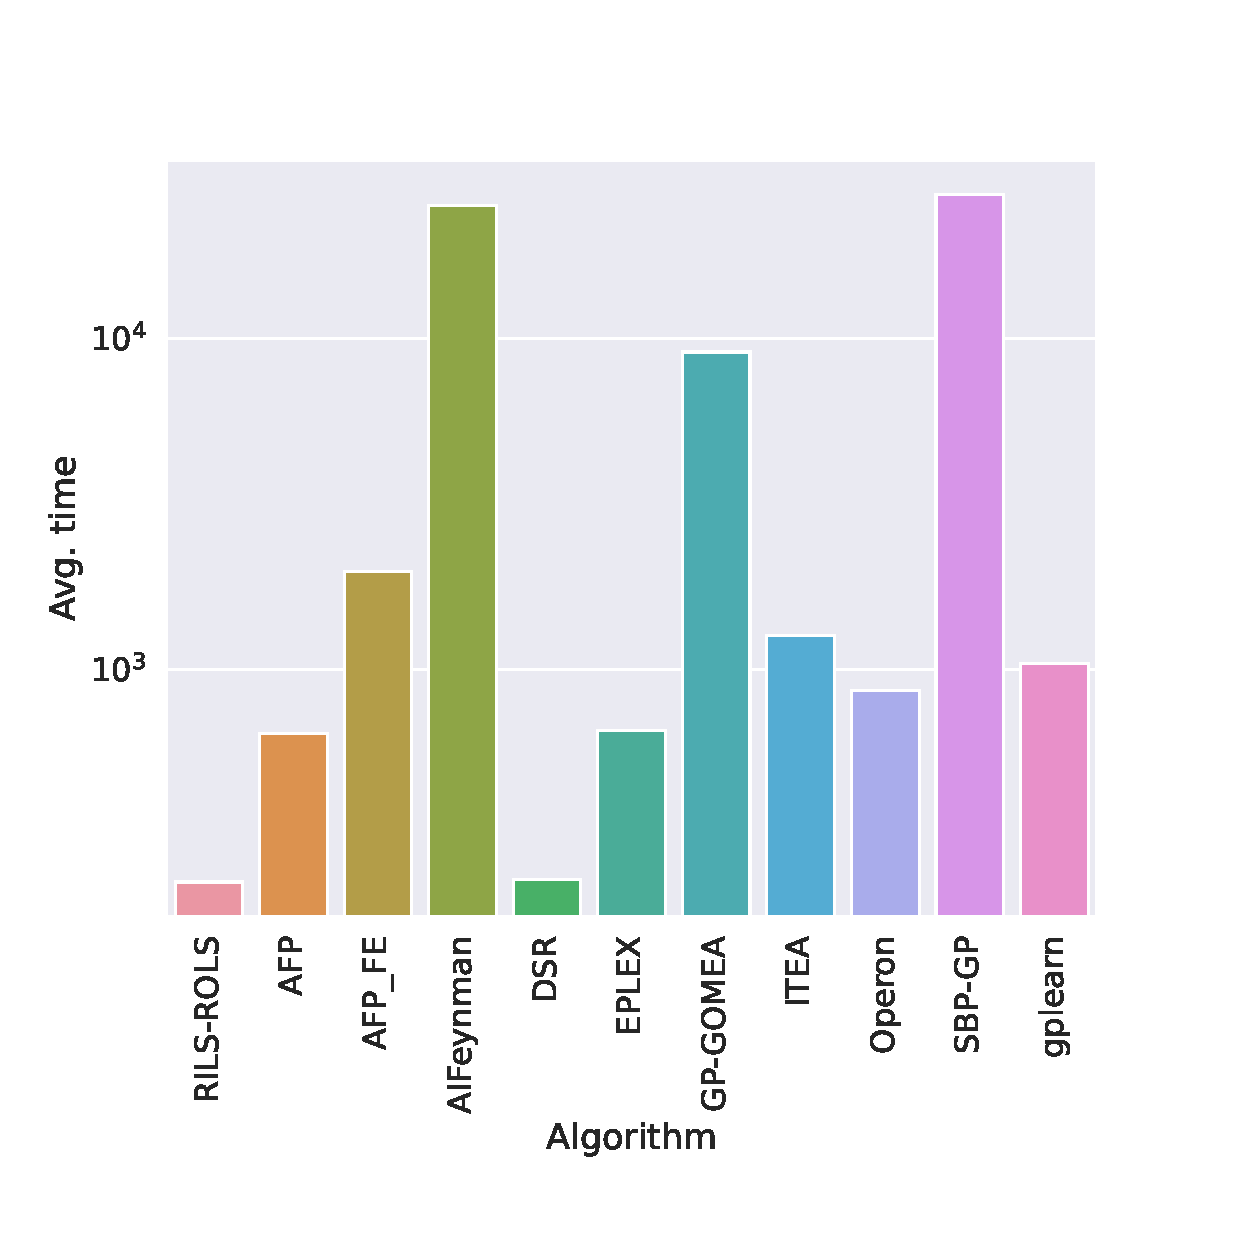
\includegraphics[  width=220pt,height=150pt]{plots/time-avg-noise0.0.eps}
		\caption{No noise}
		\label{fig:noNoise-time}
	\end{subfigure}
	\hfill
	\begin{subfigure}[b]{0.45\textwidth}
		
		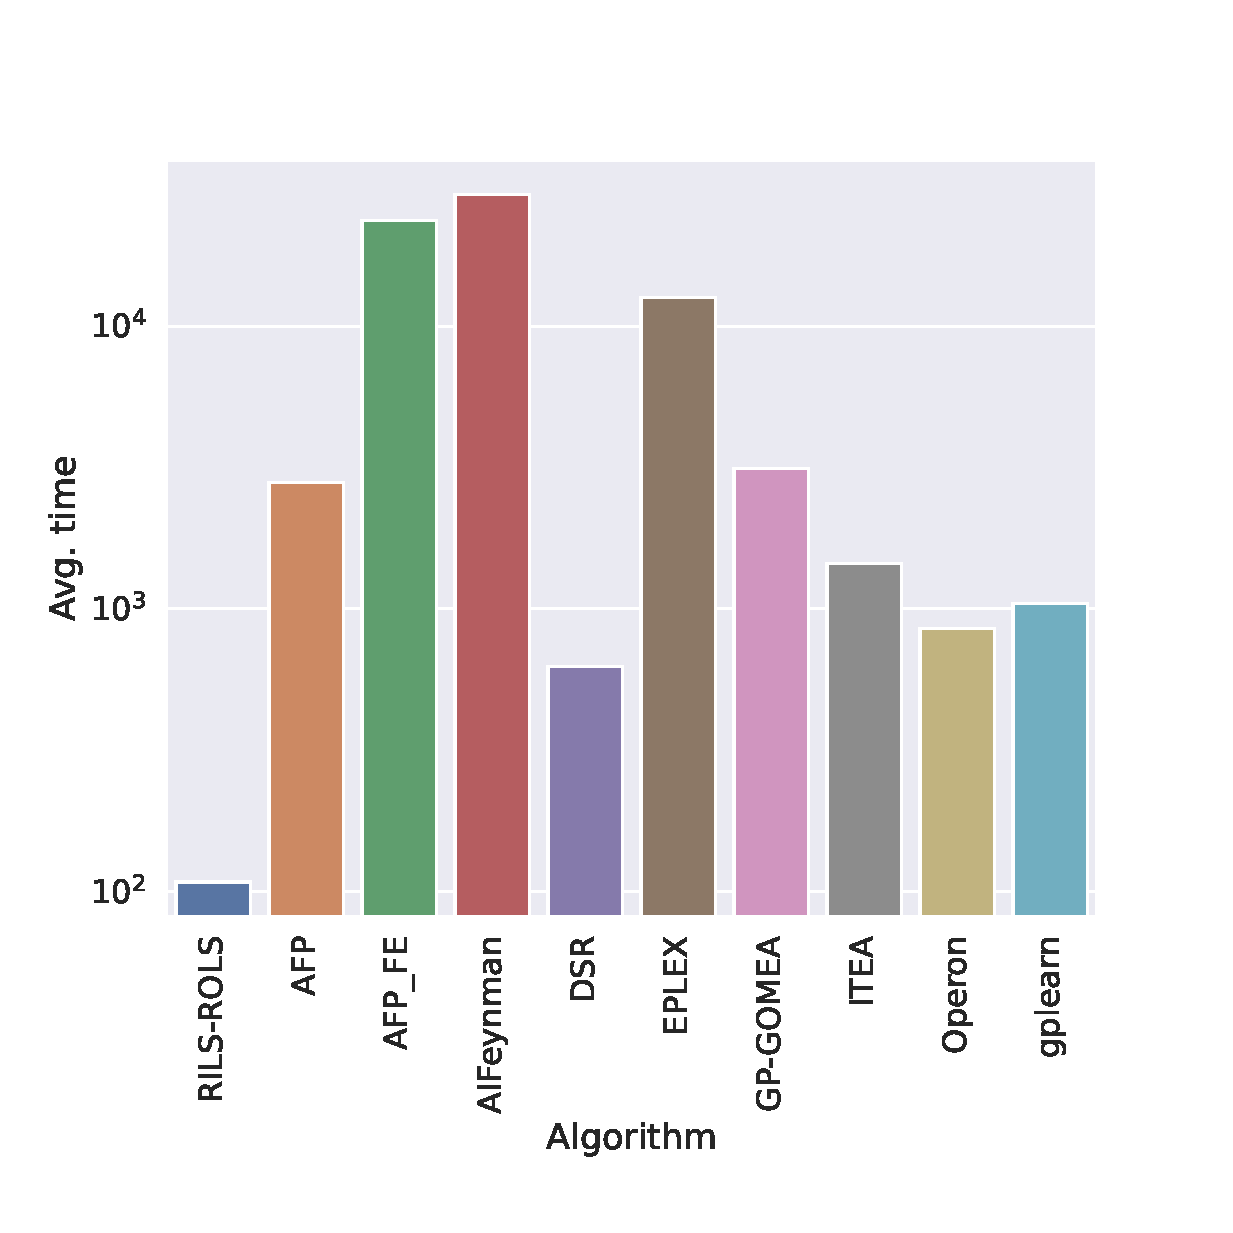
\includegraphics[  width=220pt,height=150pt]{plots/time-avg-noise0.001.eps}
		\caption{Level of noise equal to 0.001}
		\label{fig:noise0.001-time}
	\end{subfigure}
	\centering
	\begin{subfigure}[b]{0.45\textwidth}
		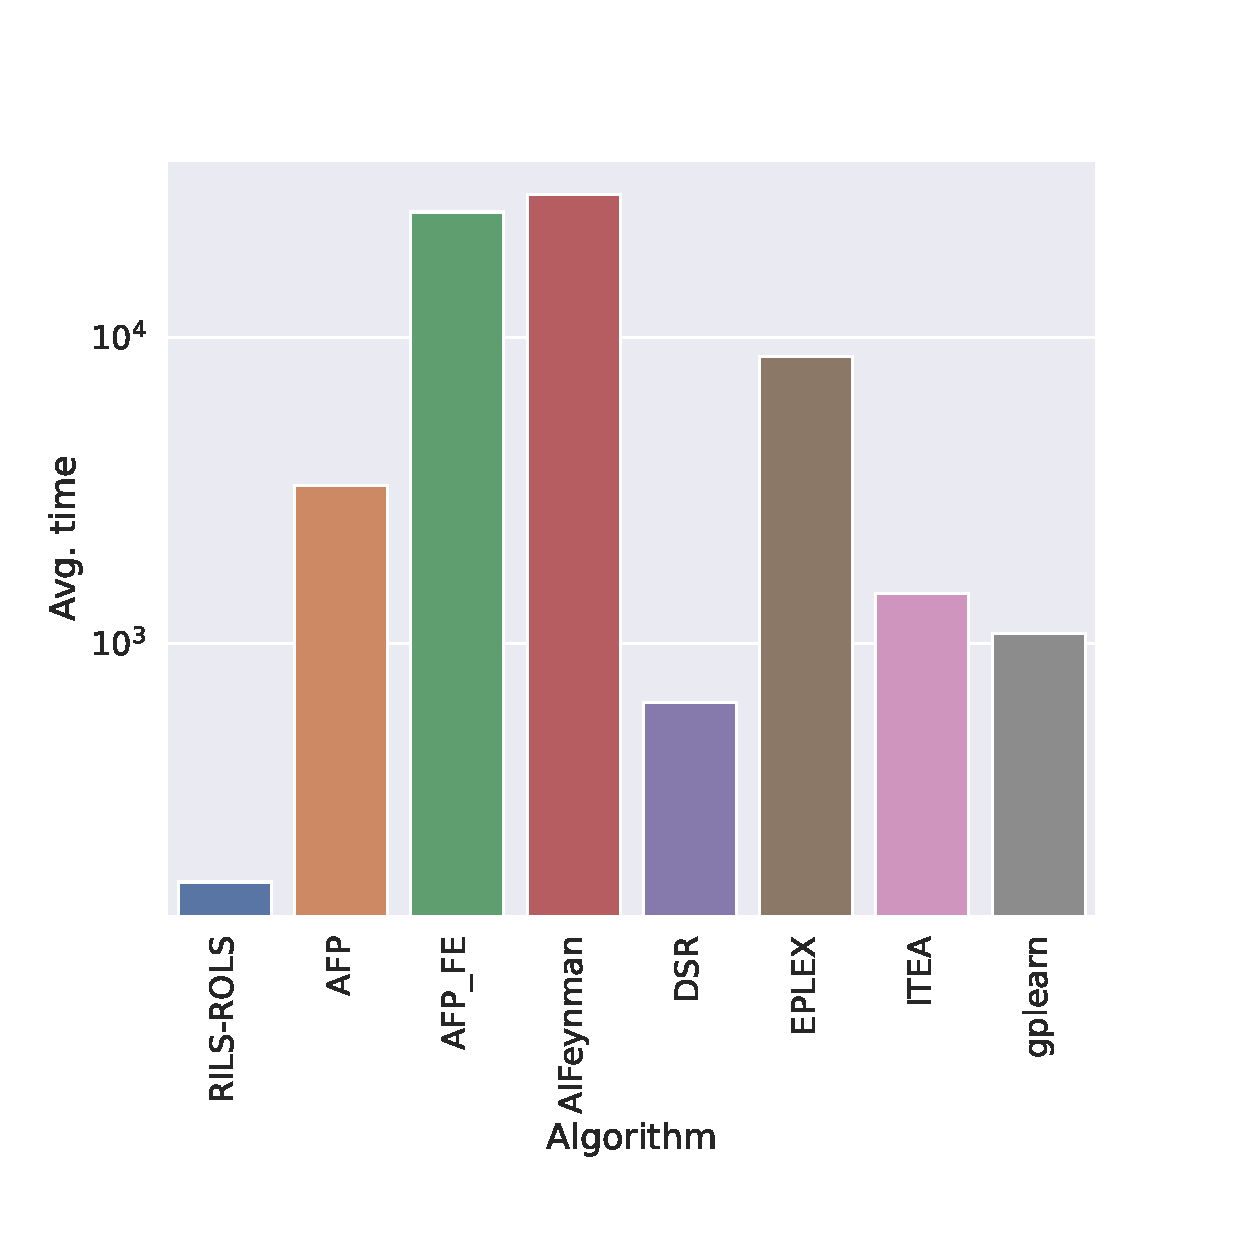
\includegraphics[  width=220pt,height=150pt]{plots/time-avg-noise0.01.eps}
		\caption{Level of noise equal to 0.01.}
		\label{fig:noise0.01-time}
	\end{subfigure}
	\caption{Average runtimes on the instance problems where the exact solution has  been reached (considered only those algorithms whose the exact percentage is at least 5\% of all runs).}
	\label{fig:time-avg-exact-noise}
\end{figure}

In Figure~\ref{fig:time-avg-exact-noise}, average runtimes of the algorithms on those instance problems from the both ground-truth benchmarks for which the exact model has  been found are compared. Those algorithms which obtained an exact percentage of at least 5\% (considering all 1300 runs) are considered as relevant here and therefore included into comparisons.  The results are grouped varying different (three) levels of noise, each presented by a plot, where the algorithms are labelled on $x$-axis, while respective average runtimes are shown on $y$-axis. Note that $y$-axis is logarithmically scaled. The following conclusions are drawn from here.

\begin{itemize}
	\item When considering the instance problems where no noise is detected, the lowest average runtime  is reported for \textsc{Rils}-\textsc{Rols} algorithm (228$s$). A slightly worse runtime is obtained by \textsc{Dsr} algorithm (232$s$).  However, note that the exact percentage of \textsc{Rils}--\textsc{Rols} is far better from \textsc{Dsr} (60.62\% vs. 19.71\%). 	All remaining approaches deliver an order of magnitude larger average runtimes that that of the \textsc{Rils}--\textsc{Rols} method. 
	\item  When considering the instance problems where a noise level of 0.001 is included,    the lowest average runtime  is again obtained by \textsc{Rils}-\textsc{Rols} algorithm (108$s$). The second best average runtime is obtained by \textsc{Dsr}, but this time significantly worse (622$s$) from the former algorithm. 
	\item When considering the instance problems with a noise level of 0.01, a similar conclusion may be drawn as that from the previous point. 
\end{itemize}



\subsection{Statistical evaluation}

In order to check the statistical significance of the obtained exact percentages and their differences between the competitor approaches, we employed the statistical methodology comparing the results of \textsc{Rils}--\textsc{Rols} to 14 other approaches on all problem instances from the both ground-truth benchmark sets, \textsc{Feynman} and \textsc{Strogatz}. Note that an indicator random variable is involved per each run of the algorithms. Thus, the score that comes into the statistical observation is an indicator (0 or 1) indicating weather or not an algorithm was able to return the exact model within  considered run. Thus, we involved 1300 results into our statistical evaluation per each algorithm. Note that at some cases some of the 14 competitors are not known from \url{https://cavalab.org/srbench/results/} due to some reasons. For these cases, we simply count a 0 as the score.   

Initially, Friedman’s test was separately executed for all competitor approaches.      In those cases in which the null hypothesis $H_0$ was rejected ($H_0$ states that there are no statistical differences between the obtained results of all competitors) pairwise comparisons are further performed by using the Nemenyi post-hoc test~\cite{pohlert2014pairwise}. The outcome is represented by means of critical difference (CD) plots. In each CD plot, the (15) competitor approaches are placed on the horizontal axis according to their average ranking. Thereafter, the CD score is computed for a significance level of 0.05. If the difference is small enough, meaning that no statistical difference is detected, a horizontal bar linking statistically equal approaches is drawn.   The corresponding three (one for each level of noise) CD plots are shown in Figure~\ref{fig:cd-plots-exact-pcts}. The following conclusions may be drawn from there.

\begin{itemize}
	\item  Concerning the instance problems where no noise is included, \textsc{Rils}-\textsc{Rols} method returns the best average ranking in terms of obtained exact models.  The second best average ranking is achieved by \textsc{AI-Feynman} algorithm. There is  statistically significant difference between these two approaches w.r.t.\ number of found exact models. The third best approach is \textsc{Apf-Fe},  which is far behind \textsc{Rils}-\textsc{Rols} w.r.t.\ delivered average raking.  
	\item    Concerning the instance problems with the  level of noise equal to 0.001, \textsc{Rils}-\textsc{Rols} method again obtains the best average ranking in terms of the found exact models.   The second best ranking is obtained by \textsc{AI-Feynman} algorithm. There is again a statistically significant difference between the results obtained by these two approaches. The third best approach is \textsc{Afp-Fe} which perform statistically worse from \textsc{AI-Feynman}.  
	\item  Concerning the instance problems with the noise level of  0.01, again, \textsc{Rils-Rols} method produces the best average ranking according to obtained exact models; the second best approach w.r.t.\ average ranking is \textsc{Afp-Fe}, followed by \text{Dsr}, and \textsc{Afp}. These latter three approaches perform statistically equal, but significantly worse than \text{Rils}-\textsc{Rols} method. 	The fourth best approach according to its average ranking is \textsc{AI-Feynman} which is on pair with \textsc{gplearn}. Note that the average ranking of \textsc{AI-Feynman} method declines by increasing  the level of noise in the input data. Thus, despite being efficient on no-noisy data, it seem that \textsc{AI-Feynman} is very sensitive to the noise, which is not that dramatically conspicuous with our \textsc{Rils}-\textsc{Rols} method.   
	
	 \fxnote{Marko: update text}
\end{itemize}


\begin{figure}[!ht]
	\centering
	\begin{subfigure}[b]{0.40\textwidth}
		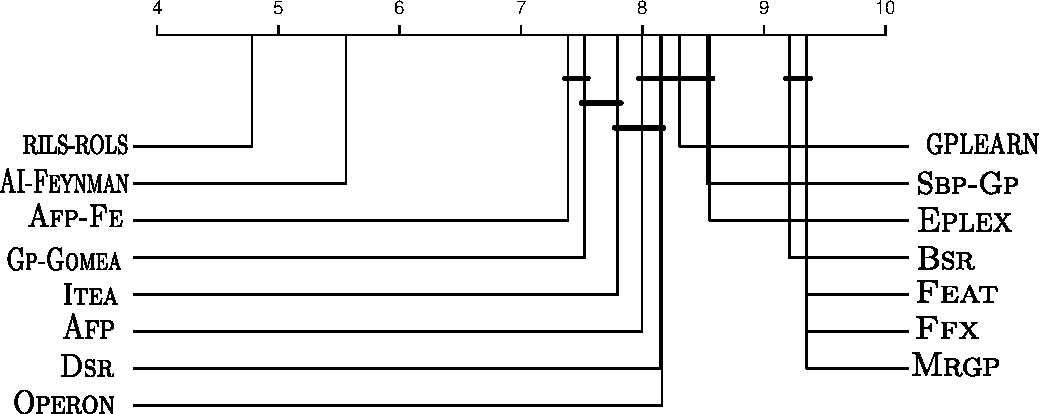
\includegraphics[  width=320pt,height=180pt]{plots/Feynman_strogatz_noise_0_0-expanded.pdf}
		\caption{No noise}
		\label{fig:CDplots-no-noise}
	\end{subfigure}
	
	\begin{subfigure}[b]{0.4\textwidth}
		
		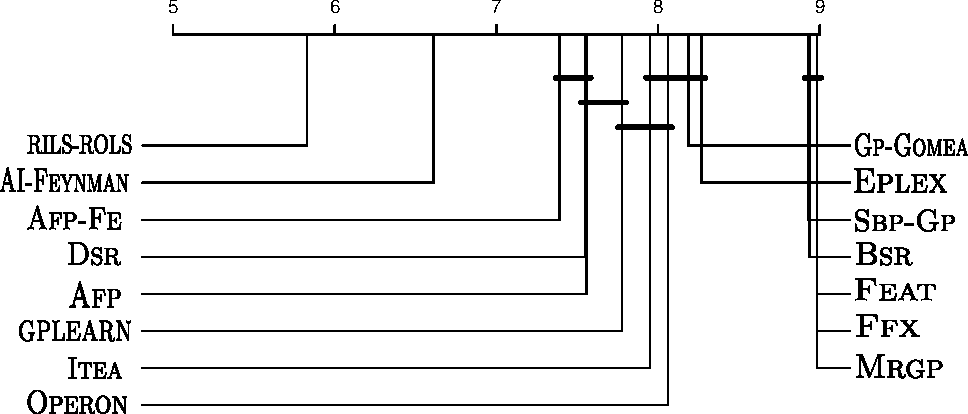
\includegraphics[  width=290pt,height=180pt]{plots/Feynman_strogatz_noise_0_001-expanded.pdf}
		\caption{Level of noise equal to 0.001}
		\label{fig:CDplots-noise0.001}
	\end{subfigure}
	
	\begin{subfigure}[b]{0.40\textwidth}
		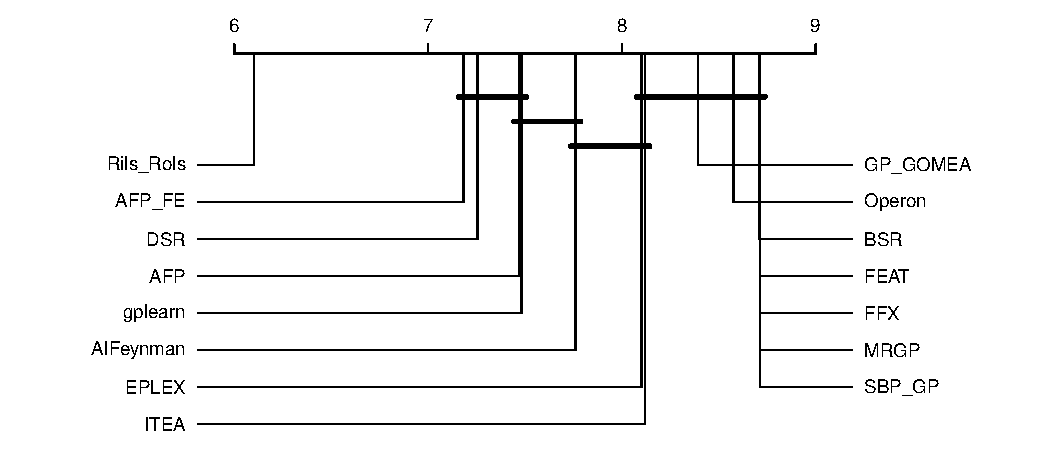
\includegraphics[  width=290pt,height=180pt]{plots/Feynman_strogatz_noise_0_01-expanded.pdf}
		\caption{Level of noise equal to 0.01.\fxnote{polish labels}}
		\label{fig:CDplots-noise0.01}
	\end{subfigure}
	\caption{CD plots comparisons in terms of exact percentages over all problem instances from the both ground-truth benchmark sets,  varying levels of noise. \fxnote{Polish labels}}
	\label{fig:cd-plots-exact-pcts}
\end{figure}


\subsection{Scalability of \textsc{Rils}-\textsc{Rols} algorithm}\label{sec:scalability-rils-rols}

In this section we study the scalability of our method in terms of the size of  instance problems and  the presence of different noise level in the input data. 

First, we divide our benchmark sets into three parts as follows. 
\begin{itemize}
	\item \textit{Small--sized instances}: all instances from \textsc{Random} benchmark whose the corresponding exact models tree representations have from 3 to 7 nodes belong to this sub-set.
	\item \textit{Middle--sized instances}:  all instances from \textsc{Random} benchmark whose the corresponding exact models tree representations have from 8 to 11 nodes belong to this sub-set.
	\item \textit{Large--sized instances}: all instances from \textsc{Random} benchmark whose the corresponding exact models tree representations have from 12 to 15 nodes belong to this sub-set. 
\end{itemize}

The results are displayed in Figure~\ref{fig:compExact_noise_size}, grouped with accordance to the (three) formed sub-groups ($x$-axis); for each of them the exact percentage rate of success of \textsc{Rils}--\textsc{Rols} algorithm is shown ($y$-axis). The following conclusions may be drawn from here:

\begin{itemize}
	\item   As expected, the exact percentage success rate is the highest for the small--sized instance problems; it is sightly bellow 90\% for the no-noisy data. For noisy data, the success rate of the algorithm gets decreased as the level of noise increases. For example, on the small-sized problem instances with the noise level  of 0.0001, and 0.01, the exact percentage of \textsc{Rils}--\textsc{Rols} is still reasonably high, at about 55\%~ and 34 \%, respectively. 
	\item For the middle-sized instance problems, the exact percentage rate is slightly bellow 50\%. It also decreases by increasing the level of noise in the target data; for the highest level of noise (of 0.01), the success rate of \textsc{Rils}-\textsc{Rols} method is just about 6\%. 
	\item For the large-sized instance problems with no noise is utilized, the exact percentage of \textsc{Rils}--\textsc{Rols} algorithm is at about 25\%, which means that the increase in the size of exact models affects the algorithm's performance, but within the expected range.  
	
	\item From the above, we can conclude that the size of exact models (solutions) and the increase of the noise level both contribute to overall performance of our \textsc{Rils}--\textsc{Rols} method. The exact percentage rate of the algorithm seems decreasing linearly  in the (exact) model size, regardless of the noise level values.
	
	\item Concerning the high--accuracy percentages delivered by \textsc{Rils}--\textsc{Rols} algorithm -- that is the percentage of problem instances for which the algorithm's termination yielded a model with $R^2 \geq 0.999$ -- for the small--sized problem instances with no noise is recorded, it is almost at the perfect score (i.e. $\approx$100\%). In the presence of a low noise level (equals to 0.001), the percentages of instance problems with the high--accuracy is still high, at about 95\%. In case when the high level of noise (equals to 0.01) is presented in the input data, these percentages stagnate, but still are at a respectable 66\%. %small-sized instances it reaches a high--precision of $R^2=0.999$ upon termination.   
	As we pointed out already, a half of these math to the respectable exact models.
	
	\item Concerning the high--accuracy percentage of the \textsc{Rils}--\textsc{Rols} algorithm on the middle-sized instance problems when the input data are free of the noise, it is obtained on 65\% cases.    The noisy the data are, the accuracy percentages of the algorithm, as expected, drop off; however, not so dramatically. For the level of noise of 0.01, the high--accuracy of the final solution is reported on $\approx$30\% cases.
	
	\item Concerning the high--accuracy percentages of the \textsc{Rils}--\textsc{Rols} algorithm on the large-sized instance problems with no noise, it gets 60\%. Not so surprisingly, the hardest case to obtain the desired high--accuracy (that is, ensuring $R^2\geq 0.999$ for the outcome  upon termination) is in the presence of a high level of noise (of 0.01), where the algorithm was successful on about 20\% of the considered large--sized instance problems. 
	
\end{itemize}

\begin{center}
	\begin{tikzpicture}
		\begin{axis}[
			xlabel=\textbf{model size},
			ylabel=\textbf{exact percentage},
			xmin=0, xmax=4,
			ymin=0, ymax=100,
			xtick={1,2,3},
			xticklabels={small,medium,large},   % <---
			ytick={0,10,...,100}
			]
			\addplot[smooth,mark=*,blue] plot coordinates {
				(1,85)
				(2,42.5)
				(3,21.05)
			};
			\addlegendentry{No noise}
			
			\addplot[smooth,color=red,mark=x]
			plot coordinates {
				(1,51.67)
				(2,13.75)
				(3,5.26)
			};
			\addlegendentry{Noise level 0.001}
			
			\addplot[smooth,color=green,mark=o]
			plot coordinates {
				(1,31.67)
				(2,5)
				(3,4.21)
			};
			\addlegendentry{Noise level 0.01}
		\end{axis}
	\end{tikzpicture}
	\captionof{figure}{Exact solution percentages for varying levels of noise and formulae sizes}
	\label{fig:compExact_noise_size}
\end{center}

\begin{center}
	\begin{tikzpicture}
		\begin{axis}[
			xlabel=\textbf{model size},
			ylabel=\textbf{$R^2 > 0.999$ percentage},
			xmin=0, xmax=4,
			ymin=20, ymax=100,
			xtick={1,2,3},
			xticklabels={small,medium,large},   % <---
			ytick={20,30,...,100}
			]
			\addplot[smooth,mark=*,blue] plot coordinates {
				(1,98.33)
				(2,62.5)
				(3,58.95)
			};
			\addlegendentry{No noise}
			
			\addplot[smooth,color=red,mark=x]
			plot coordinates {
				(1,93.33)
				(2,53.75)
				(3,40)
			};
			\addlegendentry{Noise level 0.001}
			
			\addplot[smooth,color=green,mark=o]
			plot coordinates {
				(1,65)
				(2,31.25)
				(3,20)
			};
			\addlegendentry{Noise level 0.01}
		\end{axis}
	\end{tikzpicture}
	\captionof{figure}{Percentages of solutions having $R^2 > 0.999$ for varying levels of noise and formulae sizes}
	\label{fig:compR2_noise_size}
\end{center}

In this paragraph we investigate the  scalability of our \textsc{Rils}--\textsc{Rols} algorithm in terms of the number of variables and sizes of corresponding exact models of the problem instances varying levels of noise. There is three bar plots shown per each level of noise.  These are shown by Figures~\ref{fig:compExact_noise_varcnt} and~\ref{fig:compExact_noise_varsizes}. The instances are grouped according to the different variable count/size of respective exact models ($x$-axis). For each group, the exact percentages of success rate of \textsc{Rils}--\textsc{Rols} algorithm on the instance group is shown ($y$-axis).

The following conclusions can be drawn from Figure~\ref{fig:compExact_noise_varcnt}. 

\begin{itemize}
	\item The exact percentage rate of \textsc{Rils}--\textsc{Rols} algorithm  slightly decrease as the expected number of variables gets larger when no noise is presented in the data.
	\item The exact percentages drop off with the presence of a larger noise level. Thus, the higher the noise level, the smaller the exact percentages are.
	\item Interestingly, in the presence of noise, the highest exact percentages are not obtained on the problem instances whose exact models consists of a single variable, but two or three. We argue it by the fact that the early phase of the algorithm will more likely try to include additional variables in the solution at the cost of increasing the model accuracy to ensure improving the fitness value over iterations. In the presence of the zero noise, OLS method will more likely find a smaller model (on $\approx$ 50\% cases) with a high accuracy that fits to the (no-noisy) input data than the case of noisy data. When the data is noisy, the decision of adding more variables at the beginning is likely to be forced than just dealing with short-size solutions. By the algorithm's progression, it gets harder improving the best fitness value by adding variables, and other operations are more frequently involved than in previous iterations. %This conclusion also correlates to the shape of fitness function given by Equation~(\ref{eq:fitness}) where the first two product terms there are already small (close to 1).      \fxnote{TODO: need to be further expanded...}
	%Obtaining an accurate model with a few variables in the presence of a high level of nose in the data 
\end{itemize}

\begin{figure}[!ht]
	
	
	\begin{subfigure}[b]{0.40\textwidth}
		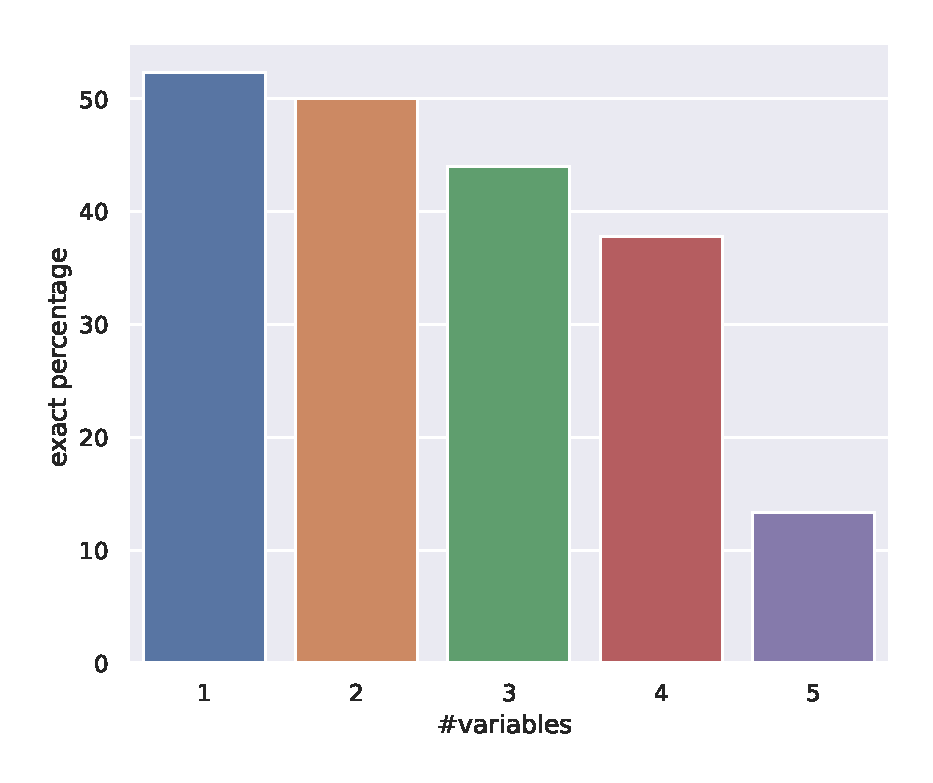
\includegraphics[  width=180pt,height=140pt]{plots/numvars_vs_exact_correct_no_noise.eps}
		\caption{No noise}
		\label{fig:noNoise}
	\end{subfigure}
	\hfill
	\begin{subfigure}[b]{0.4\textwidth}
		
		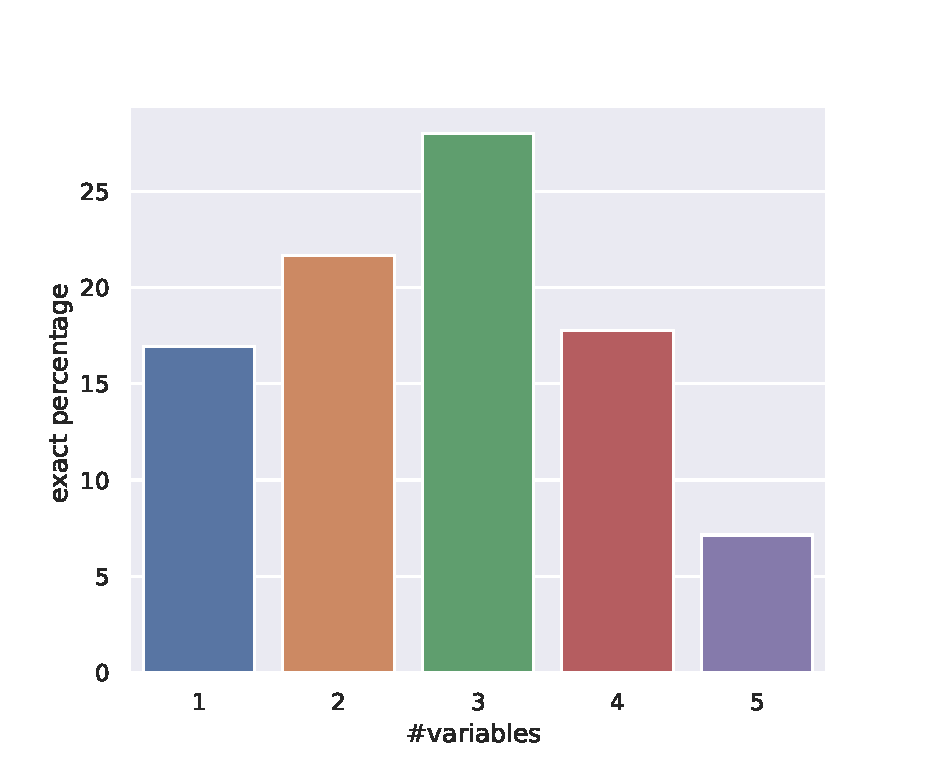
\includegraphics[  width=180pt,height=140pt]{plots/numvars_vs_exact_correct_noise0_001.eps}
		\caption{Level of noise equal to 0.001}
		\label{fig:noise0.001}
	\end{subfigure}
	\centering
	\begin{subfigure}[b]{0.40\textwidth}
		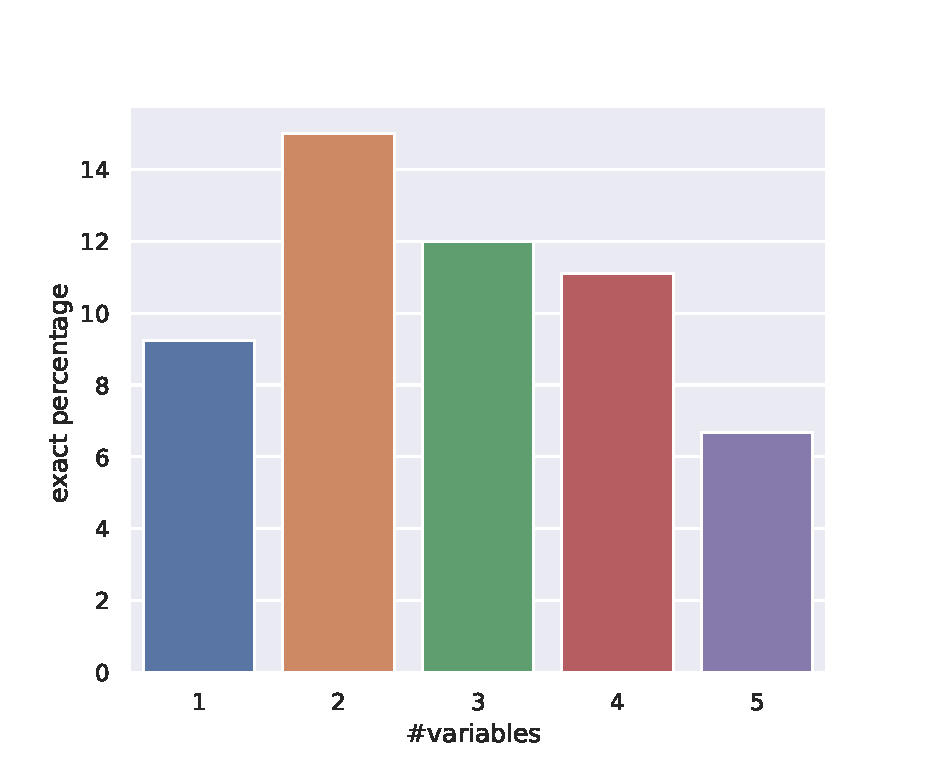
\includegraphics[  width=180pt,height=140pt]{plots/numvars_vs_exact_correct_noise0_01.eps}
		\caption{Level of noise equal to 0.01.}
		\label{fig:noise0.01}
	\end{subfigure}
	\caption{Exact solution percentages for varying levels of noise and variable counts.}
	\label{fig:compExact_noise_varcnt}
\end{figure}

The  following conclusions may be drawn from Figure~\ref{fig:compExact_noise_varsizes}.
\begin{itemize}
	\item The exact percentages are decreased with the increase of size of exact models, in case of any level of noise utilized on the target values.  %within the input data.
	\item The highest exact percentages, which are higher than 70\%, are noticed for the small-sized problem instances  (the size ranges from 3 to 7) exact models. However, for the same sizes, for noisy data, these percentages are significantly lower; for example, in case of models of size 7 and the level of noise of 0.001 and 0.01, the exact percentages obtained are 20\% and 10\%, respectively. 
	
	\item   For the problem instances with a largest size of (exact) models for no noisy data, exact percentages are never lower than 20\%. The opposite holds for noisy data. 
\end{itemize}

\begin{figure}[H]
	\begin{subfigure}[b]{0.40\textwidth}
		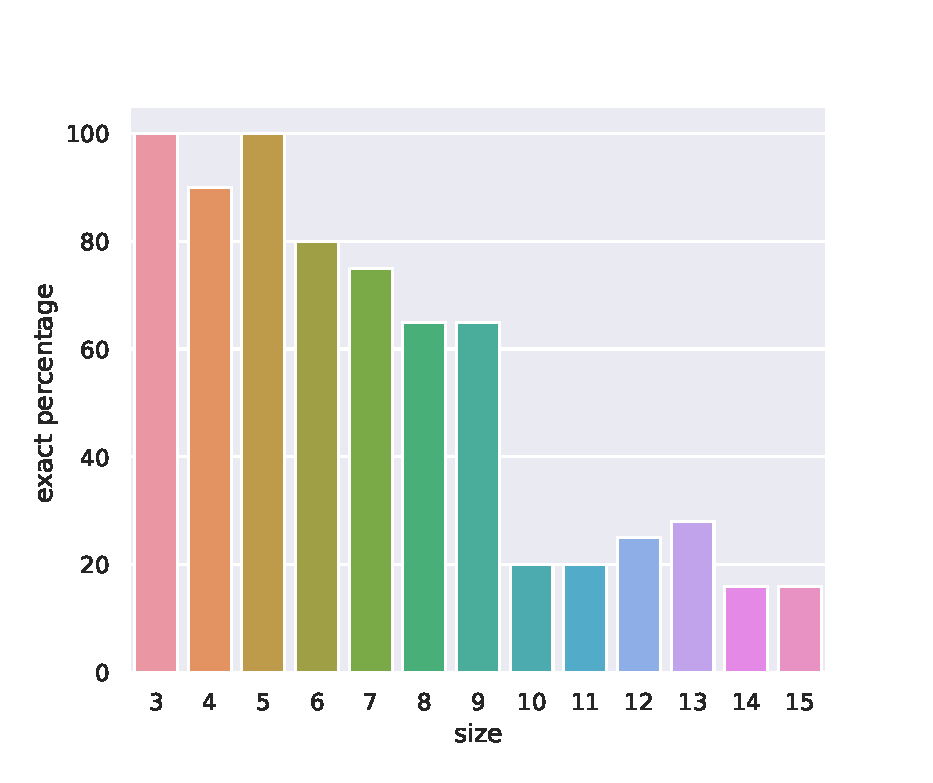
\includegraphics[  width=180pt,height=140pt]{plots/numsize_vs_exact_correct_no_noise.eps}
		\caption{No noise}
		\label{fig:size-no-noise}
	\end{subfigure}
	\hfill
	\begin{subfigure}[b]{0.4\textwidth}
		
		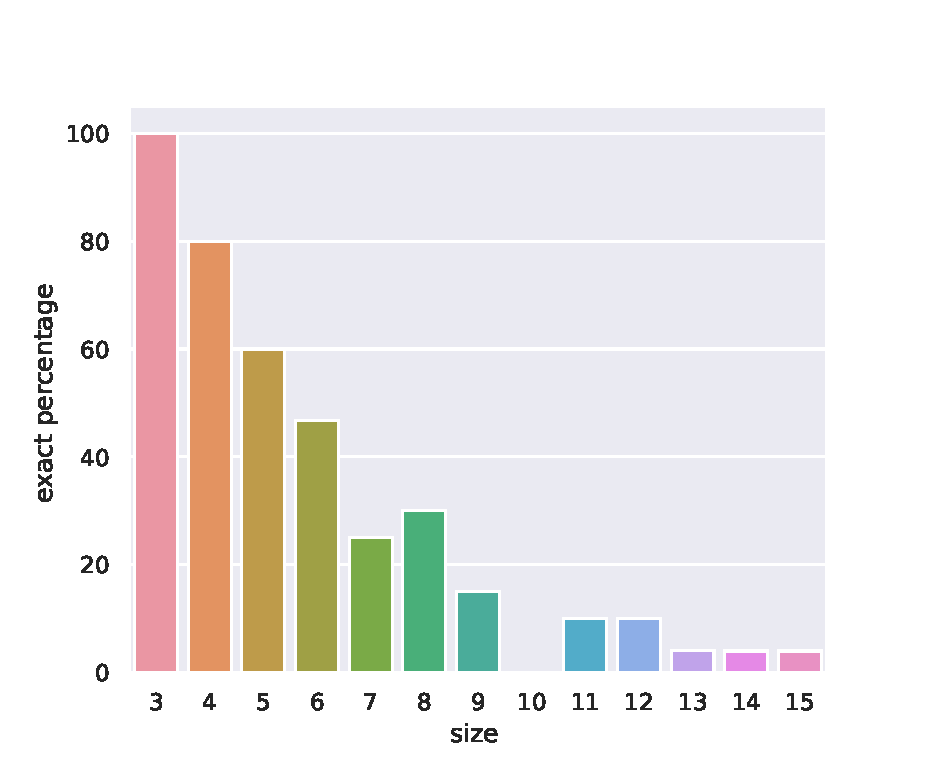
\includegraphics[  width=180pt,height=140pt]{plots/numsize_vs_exact_correct_noise0_001.eps}
		\caption{Level of noise equal to 0.001}
		\label{fig:size-noise0.001}
	\end{subfigure}
	\centering
	\begin{subfigure}[b]{0.40\textwidth}
		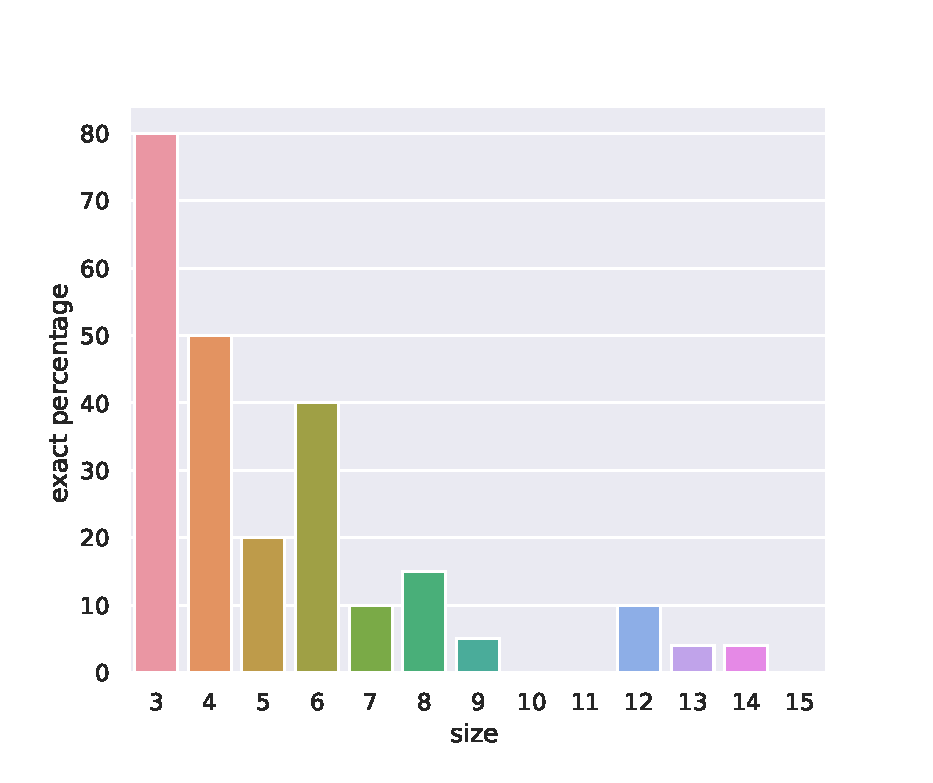
\includegraphics[  width=180pt,height=140pt]{plots/numsize_vs_exact_correct_noise0_01.eps}
		\caption{Level of noise equal to 0.01.}
		\label{fig:size-noise0.01}
	\end{subfigure}
	\caption{Exact solution percentages for varying levels of noise and exact model sizes.}
	\label{fig:compExact_noise_varsizes}
\end{figure}

When one concerns of runtime analysis of the \textsc{Rils}--\textsc{Rols} algorithm on the \textsc{Random} benchmark set w.r.t\ number of variables, the results are displayed in Figure~\ref{fig:runtime_rils_rols}. The instances are grouped w.r.t.\ number of variables included into corresponding exact model ($x$-axis). The following conclusions may be drawn from there.  

\begin{itemize}
	\item As one could expect, average runtime is getting increased with the increase of the number of variables in exact models. 
	\item Note that the average runtime in case of the instances whose exact models have the largest number of variables (5) is just about 200$s$.
	\item The two above-mentioned points indicate efficacy of our method especially in case of expected exact models of a small and middle sizes with small--to--middle levels of noise included in the input data. In these cases, the algorithm is able to deliver the reasonable exact percentages, which are always larger than 50\%. Note that models which have more compact representations (thus, small in their size) are desirable in many areas of natural sciences due to easier interpret-ability more than models represented by a more complex expression.   
\end{itemize}

\begin{figure}[H]
	\begin{subfigure}[b]{0.40\textwidth}
		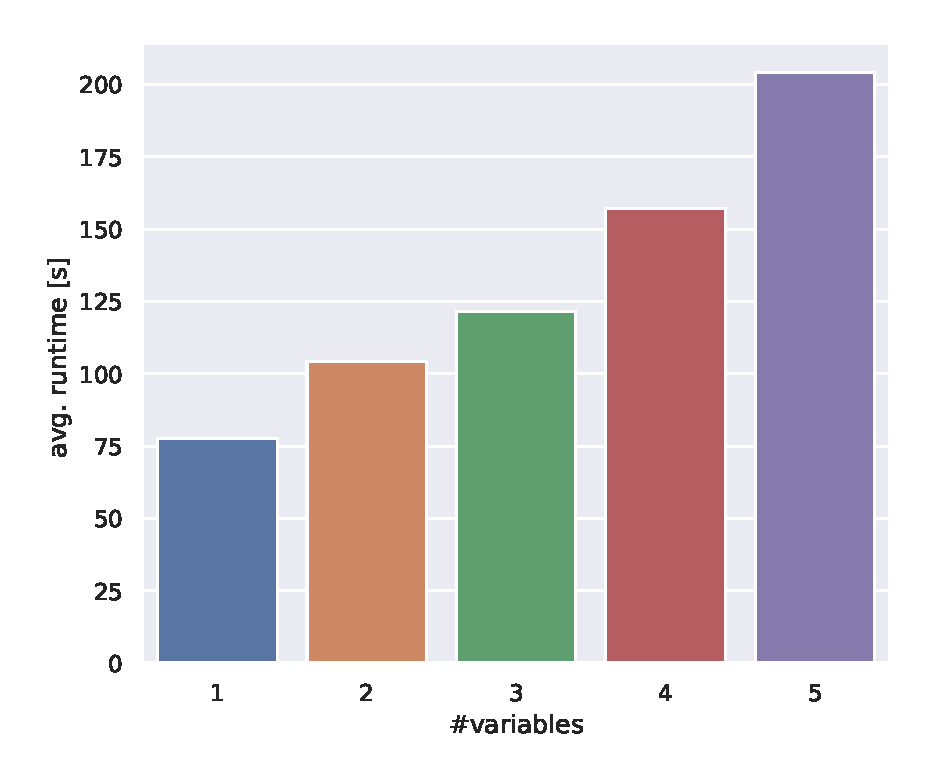
\includegraphics[  width=180pt,height=140pt]{plots/numsize_vs_time_no_noise.eps}
		\caption{No noise}
		\label{fig:time-no-noise}
	\end{subfigure}
	\hfill
	\begin{subfigure}[b]{0.4\textwidth}
		
		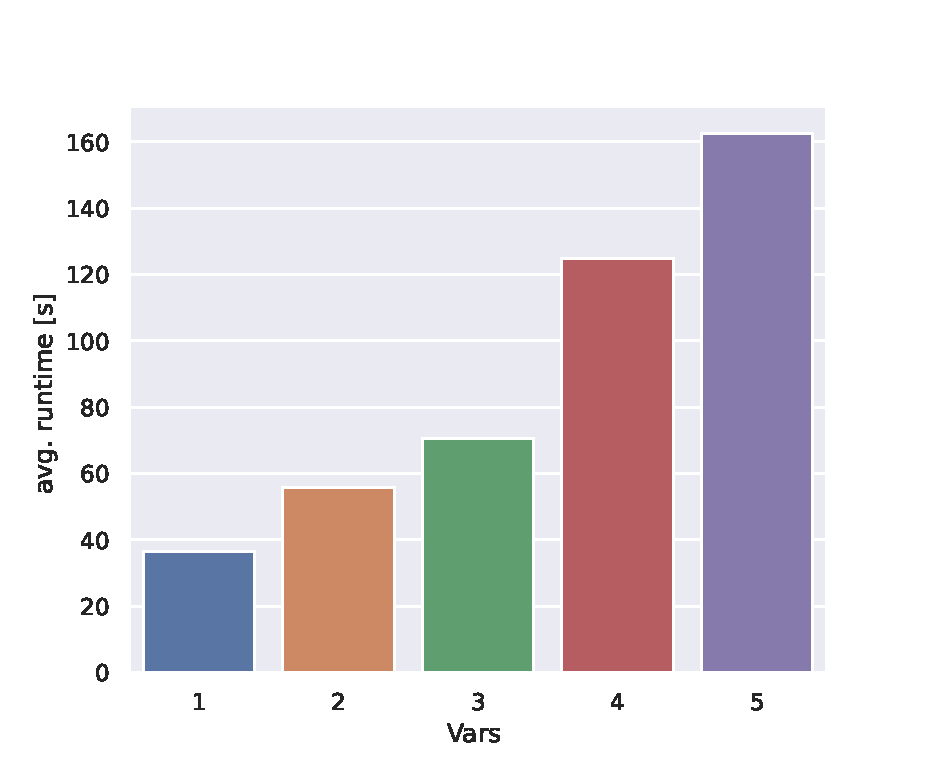
\includegraphics[  width=180pt,height=140pt]{plots/vars_vs_time_noise0_001.eps}
		\caption{Level of noise equal to 0.001}
		\label{fig:time-noise0.001}
	\end{subfigure}
	\centering
	\begin{subfigure}[b]{0.40\textwidth}
		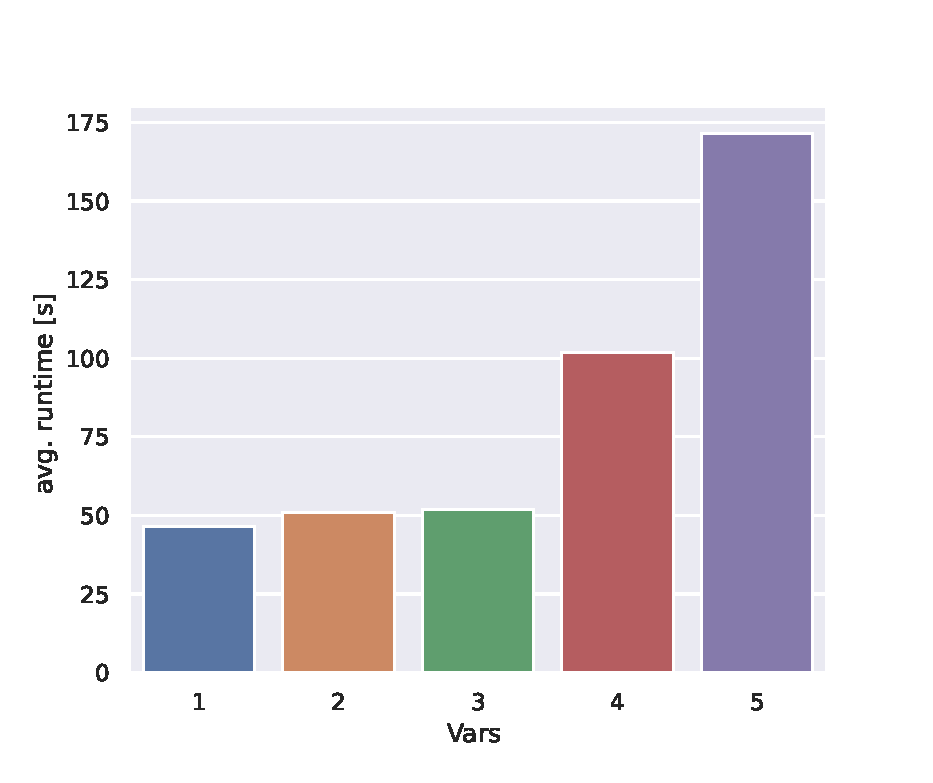
\includegraphics[  width=180pt,height=140pt]{plots/vars_vs_time_noise0_01.eps}
		\caption{Level of noise equal to 0.01.}
		\label{fig:time-noise0.01}
	\end{subfigure}
	\caption{Average runtime comparisons for varying levels of noise and variable counts.}
	\label{fig:runtime_rils_rols}
\end{figure}

\begin{comment}
	\begin{center}
		\begin{tikzpicture}
			\begin{axis}[
				xlabel=$variable\;count\;in\;exact\;models$,
				ylabel=$exact\;percentage$,
				xmin=0, xmax=5,
				ymin=0, ymax=100,
				xtick={1,2,3,4},
				xticklabels={1,2,3,4},   % <---
				ytick={0,10,...,100}
				]
				\addplot[smooth,mark=*,blue] plot coordinates {
					(1,43.33)
					(2,43.33)
					(3,46.67)
					(4,46.67)
				};
				\addlegendentry{No noise}
				
				\addplot[smooth,color=red,mark=x]
				plot coordinates {
					(1,3.33)
					(2,3.33)
					(3,26.67)
					(4,26.67)
				};
				\addlegendentry{Noise level 0.001}
				
				\addplot[smooth,color=green,mark=o]
				plot coordinates {
					(1,3.33)
					(2,3.33)
					(3,3.33)
					(4,16.67)
				};
				\addlegendentry{Noise level 0.01}
			\end{axis}
		\end{tikzpicture}
		\captionof{figure}{Exact solution percentages for varying levels of noise and variable counts (only sizes ranging from 7 to 12)}
		\label{fig:compExact_noise_varcnt}
	\end{center}
\end{comment}
%\begin{center}
%	\begin{tikzpicture}
	%		\begin{axis}[
		%			xlabel=$variable\;count$,
		%			ylabel=$exact\;percentage$,
		%			xmin=0, xmax=5,
		%			ymin=0, ymax=100,
		%			xtick={1,2,3,4},
		%			xticklabels={1,2,3,4},   % <---
		%			ytick={0,10,...,100}
		%			]
		%			\addplot[smooth,mark=*,blue] plot coordinates {
			%				(1,83.33)
			%				(2,66.67)
			%				(3,73.33)
			%				(4,46.67)
			%			};
		%			\addlegendentry{No noise}
		%			
		%			\addplot[smooth,color=red,mark=x]
		%			plot coordinates {
			%				(1,56.67)
			%				(2,63.33)
			%				(3,66.67)
			%				(4,46.67)
			%			};
		%			\addlegendentry{Noise level 0.001}
		%			
		%			\addplot[smooth,color=green,mark=o]
		%			plot coordinates {
			%				(1,23.33)
			%				(2,43.33)
			%				(3,53.33)
			%				(4,26.67)
			%			};
		%			\addlegendentry{Noise level 0.01}
		%		\end{axis}
	%	\end{tikzpicture}
%	\captionof{figure}{Percentages of solutions having $R^2 > 0.999$ for varying levels of noise and variable counts (only sizes ranging from 7 to 12)}
%	\label{fig:compR2_noise_varcnt}
%\end{center}





\section{Conclusions and future work}\label{sec:conclusions}

In this paper, we dealt with solving the well--known Symbolic regression (SR)  problem. SR problem is a generalization of more interdisciplinary known problems of linear and logistic regression.    
We proposed a meta-heuristic approach, called \textsc{Rils}-\textsc{Rols}. Our approach is built upon the Iterated local search (ILS) scheme. The first crucial concept within this scheme is utilizing the ordinary least square method to efficiently determine internal coefficients that are the best fitting to the candidate solution. Thus, the search process is primarily focused on considering already promising solutions in the continuous part of the search space rather than applying enhanced heuristics to search for those coefficients. Another key aspect is the utilization of a carefully constructed fitness function in the search, which appeared as a combination of three important scores: RMSE, $R^2$  scores and the size of the model (solution).  Last but not least, a carefully constructed local search is applied systematically exploring solutions obtained as 1--perturbations of the considered solution.  1--perturbations of a solution are based on applying the six per-node change operations on the solution's tree representation. 

\textsc{Rils-Rols} method is compared to the 14 other competitor algorithms from the literature on the two ground truth benchmark sets from literature, namely \textsc{Feynman} and \textsc{Strogatz}.  Additionally, we introduced a non-biased benchmark set of randomly generated instances, labelled by \textsc{Random}.  The experimental evaluation confirmed the efficiency of our method which produced the best average ranking results in terms of exact percentage when compared to all other competitors on the two ground-truth benchmarks in the presence of all three different levels of noise in the input data. In all cases, new best exact percentages are obtained using \textsc{Rils-Rols} method.   More in details,
our algorithm was able to obtain the right model on 60.62\%, 42.08\%, and 34.77\% problem instances in the presence of the noise level of 0.0, 0.001, and 0.01, respectively. Just for the shake of comparisons, the second best approach \textsc{AI-Feynman}, when the noise level of 0.0 and 0.001 is included, obtained an exact percentage rate of 52.65\%, and 31.89\%, respectively. In case of the highest noise level, the second best approach was \textsc{Afp-Fe}, obtaining an exact percentage rate of 20\%. Additionally, the scalability and robustness of this method are checked and confirmed on the unbiased \textsc{Random} benchmark set in terms of a few different criteria such as the size of the model, the number of variables included in exact models, and obtained average runtimes. 

In future work, one could think of constructing a hybrid of \textsc{Rils-Rols} method with some other meta-heuristics to further boost the quality of the obtained results. For example, replacing ILS scheme of \textsc{Rils-Rils} with a more general Variable neighbourhood search (VNS) scheme is a reasonable option to give it a try. VNS   utilizes a more stronger and systematic system of solutions diversification and thus escaping from local optima could be much easier.  Additionally, as proof of the efficiency and benefits of our algorithm, this tool could be applied to solving problems from various problem domains out of the area of computer science, for example from physics or chemistry, to help for setting up hypotheses or to obtain valuable insights on experimental evaluations.  

\newpage
\appendix

\section{Overview of \textsc{Rils}-\textsc{Rols}  python package}\label{sec:appendix-1}
\fxnote{TODO}

\section{Additional statistical analysis}\label{sec:appendix-2}



\begin{figure}[H]
	\begin{subfigure}[b]{0.40\textwidth}
		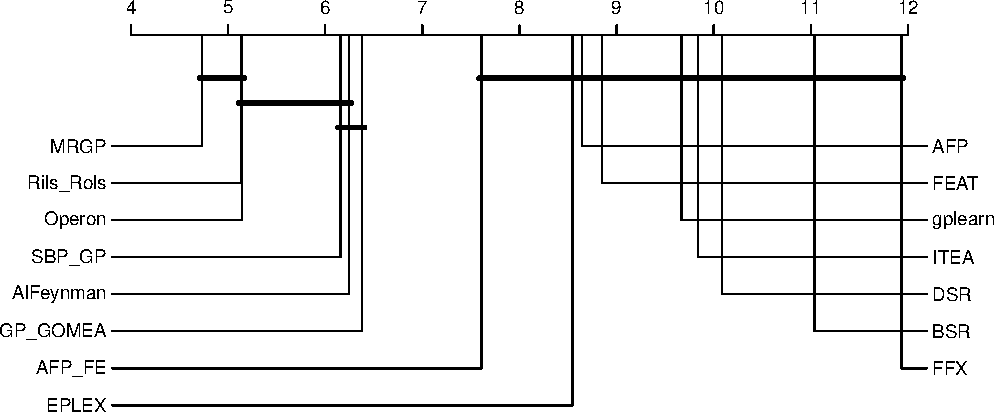
\includegraphics[  width=220pt,height=140pt]{plots/Feynman__strogatz_noise_0_0acc.pdf}
		\caption{No noise}
		\label{fig:CDplotsR2-no-noise}
	\end{subfigure}
	\hfill
	\begin{subfigure}[b]{0.4\textwidth}
		
		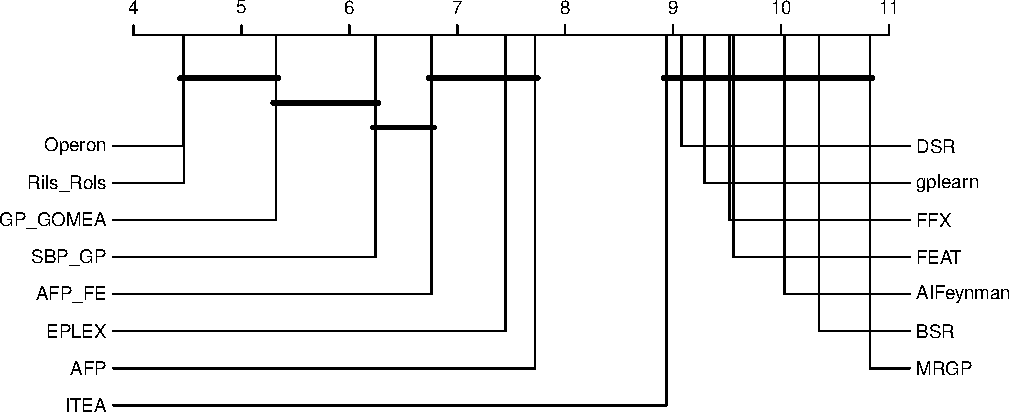
\includegraphics[  width=220pt,height=140pt]{plots/Feynman__strogatz_noise_0_001acc.pdf}
		\caption{Level of noise equal to 0.001}
		\label{fig:CDplotsR2-noise0.001}
	\end{subfigure}
	\centering
	\begin{subfigure}[b]{0.40\textwidth}
		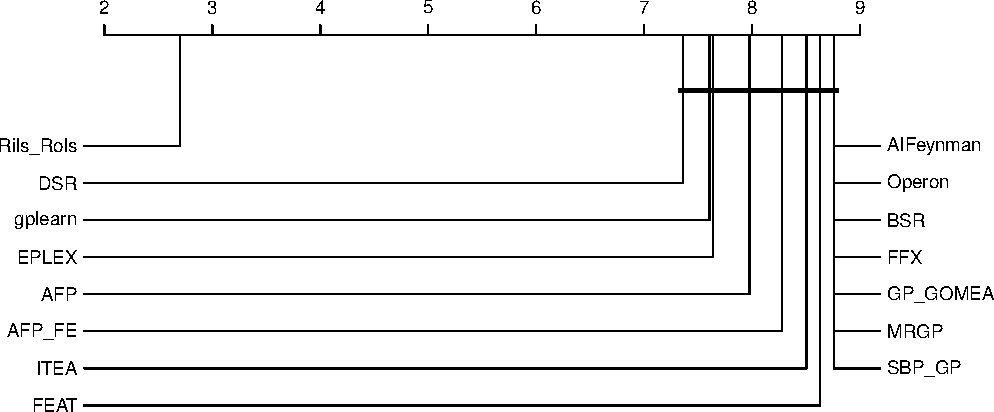
\includegraphics[  width=220pt,height=140pt]{plots/Feynman__strogatz_noise_0_01acc.pdf}
		\caption{Level of noise equal to 0.01.}
		\label{fig:CDplotsR2-noise0.01}
	\end{subfigure}
	\caption{CD plots comparisons in terms of obtained $R^2$ score over all problem instances from both ground-truth benchmark sets,  varying levels of noise.}
	\label{fig:cd-plotsR2-varying_noise}
\end{figure}


\newpage
%\section*{References}
\bibliographystyle{abbrv}	
\bibliography{bib}	


\end{document}
